\appendix
\clearpage
\addappheadtotoc
\appendixpage
	
	\chapter{Apartado A: Entrevista}
	\label{Entrevista}
	\noindent Entrevista con responsable de las actividades del Departamento de Formación Deportiva
	Buenas tardes, agradecemos el tiempo que nos esta brindando para mostrarle nuestra propuesta de Trabajo Terminal con la cual se pretende ayudar en el proceso de inscripción para los alumnos.
	
	\begin{enumerate}
		\item ¿Cuál es el proceso actual para la inscripción a un evento interpolitécnico?\\
		El alumno tiene que acudir al departamento de Actividades Deportivas de su unidad académica, informar que quiere participar en un evento inrtepolitécnico. Con esto el coordinador procede a solicitar una identificación o documento probatorio que compruebe el estatus académico del alumno, a la vez el coordinador le proporciona una cédula de inscripción para que sea llenada y entrada. Si esto cumple puede continuar con su proceso en caso contrario se detiene el trámite. En cualquiera de los dos caso el alumno es informado del resultado final.
		
		\item ¿Hay límite de edad para los participantes?
		Claro, tomando en cuenta el reglamento esta estipulado que la edad miníma de los participantes es de 18 años y la máxima es de 27 años.
		
		\item ¿Se tiene un formato definido para la inscripción?
		Actualmente no contamos con un formato en especifíco, sin embargo se trata de seguir un formato. Desafortunadamente no todos los Coordinadores de las Unidades Académicas no lo siguen de la manera correcta.\\ 
		Para nosotros esto representa mucho más tiempo para emplear al unificar el formato de la información y tratar de mitigar un poco la dificultad al buscar datos de los participantes.
		
		\item ¿Es necesario la comprobación de inscripción de los alumnos?
		Por supuesto, de igual manera tomando en cuenta el reglamento se especifíca que los alumnos solo podrán participar en un evento siempre y cuando este esté inscrito en el periodo actual al del evento de su interés.\\
		Desafortunadamente, nos hemos percatado de que se han inscrito alumnos que no cumplen con este requisito.
		
		\item ¿Cuántos deportes hay actualmente practicándose en el IPN?
		Actualmente en el Instituto Politécnico Nacional se practican 27 deportes.
		
		\item ¿Se cuenta con algún método de verificación de datos?
		No, es por esta razón que nos hemos percatado hasta el momento de hacer la publicación de resultados que se inscriben alumnos que no están inscritos o personas ajenas al mismo.
		
		\item Una vez concluido los eventos, ¿Qué sigue?
		Se realiza el pago del arbitraje de los eventos, hasta que se haga dicho pago nos es proporcionado los resultados de los participantes.\\
		Teniendo estos, procedemos a realizar el vaciado de los datos para posteriormente sea publicado y así, los participantes puedan ver su desempeño.
		
		\item ¿Cuánto tiempo suele tardarse en la publicación de los resultados?
		En el mejor de los casos nos toma al rededor de una semana, muchas veces esto depende del pago del arbitraje. En algunas ocasiones nos hemos tomado hasta un mes o mes y medio en la publicación de los resultados. 
		
		\item ¿Qué puntos se consideran en la generación de estadísticas?
		Se toman en cuenta la participación de los alumnos por escuela, posteriormente se límita a la cantidad de hombres y mujeres que participaron. También se toma en cuenta la participación por el deporte tomando en cuenta los parametros antes mencionados.
		
	\end{enumerate} 
	
	\chapter{Apartado B: Mensajes}
	\noindent En este apartado, se describen a detalle los mensajes que se encuentran dentro de la aplicación web. Estos mensajes contemplan la notificación de un proceso completado o un error en algún proceso del mismo.
		\section{Mensajes de RIDESCOM}

%===========================  MSG1 ==================================

\begin{mensaje}{MSG1}{Faltan campos por completar}{Error}

	\item[Canal:] Sistema.

    \item[Propósito:] Informar al actor que no se puede realizar el Inicio de sesión ya que no ha completado los campos requeridos.

    \item[Redacción:] Debe ingresar los datos del campo Usuario y Contraseña.

    \item[Parámetros:] Ninguno.

    \item[Ejemplo:] Usuario: Usuario, Contraseña: Contraseña.

	%\item[Referenciado por: ] \refIdElem{DIC-UA-COSIE-CU1.3}, \refIdElem{DIC-UA-COSIE-CU1.3.1},  \refIdElem{DIC-UA-COSIE-CU1.3.2}%\refIdElem{DIC-A-CU1}, \refIdElem{DIC-A-CU2}, \refIdElem{DIC-A-CU3}  \refIdElem{DIC-CGC-DPF-CU1.3}

\end{mensaje}
\newline


%===========================  MSG32 ==================================

\begin{mensaje}{MSG2}{Los datos ingresados no son correctos}{Error}
	
	\item[Canal:] Sistema.
	
	\item[Propósito:] Informar al actor que no se puede realizar el Inicio de sesión ya que los datos ingresados no coinciden con los almacenados.
	
	\item[Redacción:] Debe ingresar los datos correctos del campo Usuario y/o Contraseña.
	
	\item[Parámetros:] Ninguno.
	
	\item[Ejemplo:] Usuario: Usuario, Contraseña: Contraseña.
	
	%\item[Referenciado por: ] \refIdElem{DIC-UA-COSIE-CU1.3}, \refIdElem{DIC-UA-COSIE-CU1.3.1},  \refIdElem{DIC-UA-COSIE-CU1.3.2}%\refIdElem{DIC-A-CU1}, \refIdElem{DIC-A-CU2}, \refIdElem{DIC-A-CU3}  \refIdElem{DIC-CGC-DPF-CU1.3}
	
\end{mensaje}
	
		\pagebreak
		
	\chapter{Apartado C: Diseños de Pantallas}
	\label{diseños}
	\noindent Este apartado, se muestran los diseños de pantallas que se consideraron para incluir en el proyecto final. Se muestran los distintos módulos de cada uno de los participantes involucrados en la aplicación web.
	
		\begin{figure}[hbt!]
			\centering
			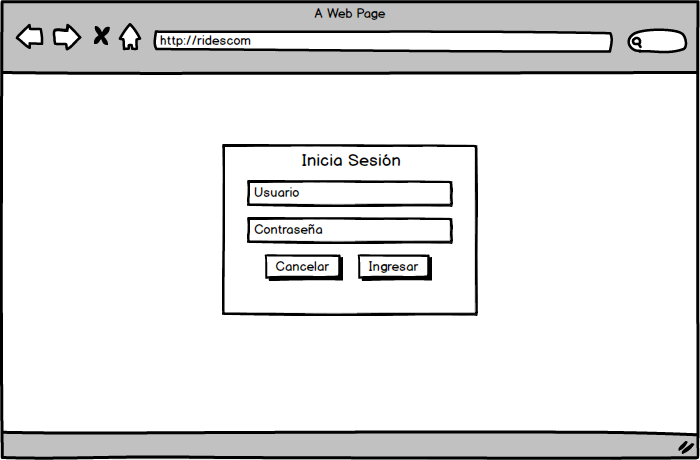
\includegraphics[width=10cm, height=6cm]{Imagenes/Nuevos/P1_LoginJFD_coord}
			\caption{Inicio sesión para el JFD y el coordinador de U.A.}
			\label{inicioJFDycoord}
		\end{figure}
		\pagebreak
		
		\begin{figure}[hbt!]
			\centering
			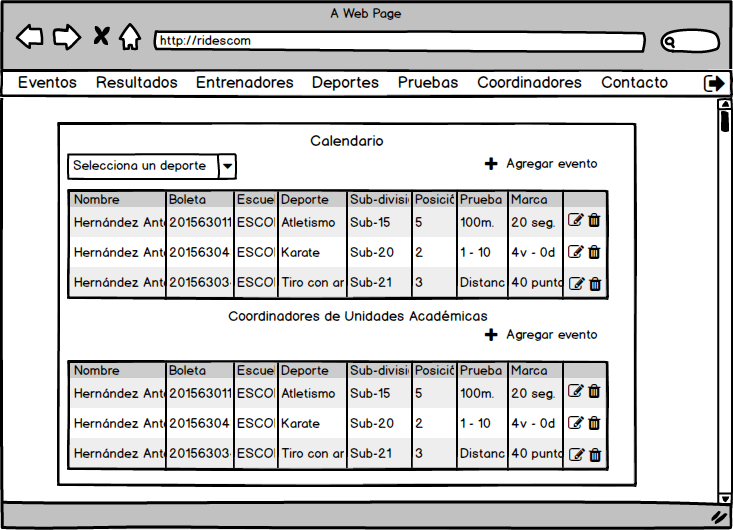
\includegraphics[width=10cm, height=6cm]{Imagenes/Nuevos/P2_Inicio_JefeFD}
			\caption{Página principal para el Jefe de Fomento Deportivo}
			\label{principalJFD}
		\end{figure}
	
		\begin{figure} [hbt!]
			\centering
			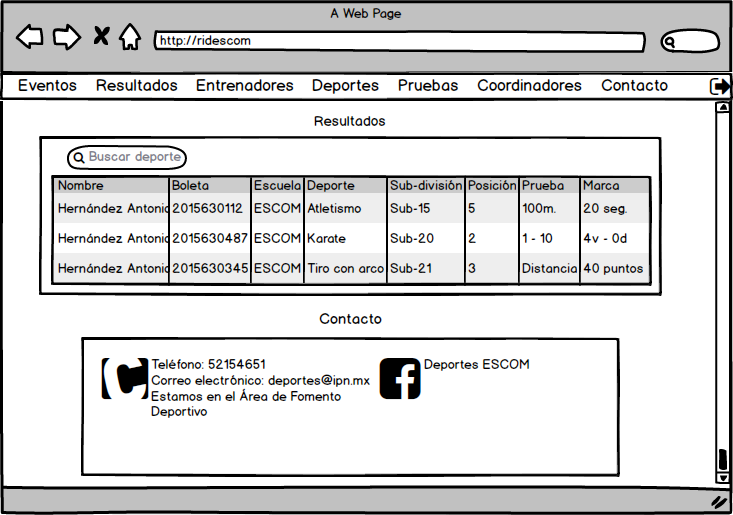
\includegraphics[width=10cm, height=6cm]{Imagenes/Nuevos/P3_Inicio_JefeFD1}
			\caption{Página principal para el Jefe de Fomento (Continuación).}
			\label{principalJFD1}
		\end{figure}
	
		\begin{figure} [hbt!]
			\centering
			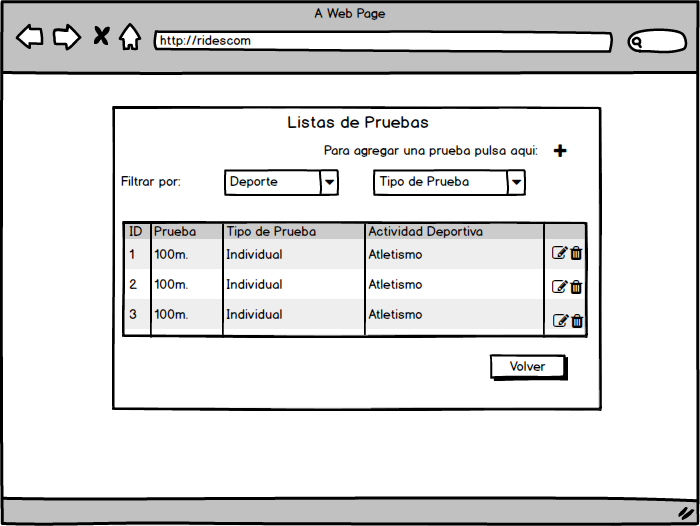
\includegraphics[width=10cm, height=6cm]{Imagenes/Nuevos/P25_Pruebas_JFD}
			\caption{Página para visualizar las pruebas dadas de alta. (Jefe de Fomento Deportivo)}
			\label{pruebas}
		\end{figure}
		\pagebreak
		
		\begin{figure} [hbt!]
			\centering
			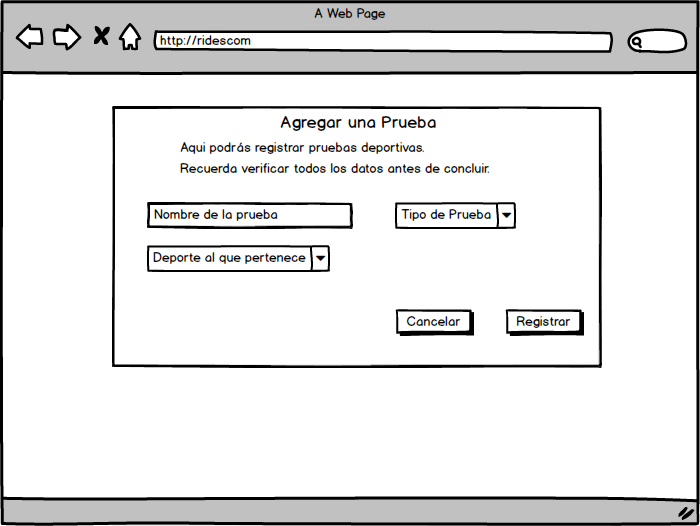
\includegraphics[width=10cm, height=6cm]{Imagenes/Nuevos/P26_AgregarPruebas_JFD}
			\caption{Página para agregar las distintas pruebas pruebas. (Jefe de Fomento Deportivo)}
			\label{agregarpruebas}
		\end{figure}
		
		\begin{figure} [hbt!]
			\centering
			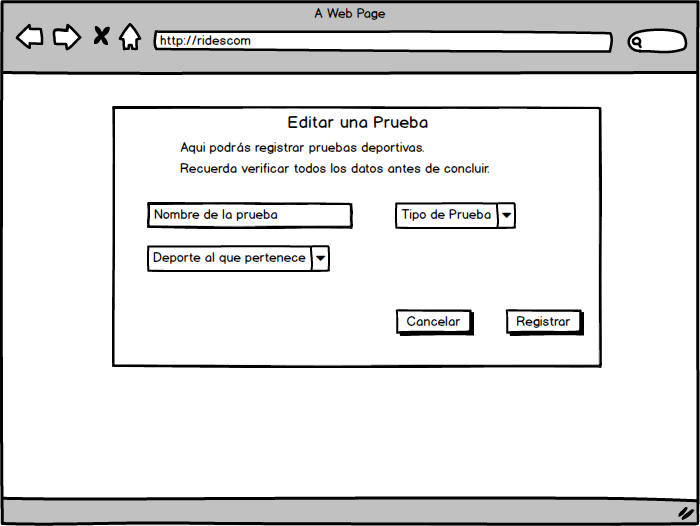
\includegraphics[width=10cm, height=6cm]{Imagenes/Nuevos/P26_EditarPruebas_JFD}
			\caption{Página para editar los datos de las pruebas previamente registrados. (Jefe de Fomento Deportivo)}
			\label{editarpruebas}
		\end{figure}
	
		\begin{figure} [hbt!]
			\centering
			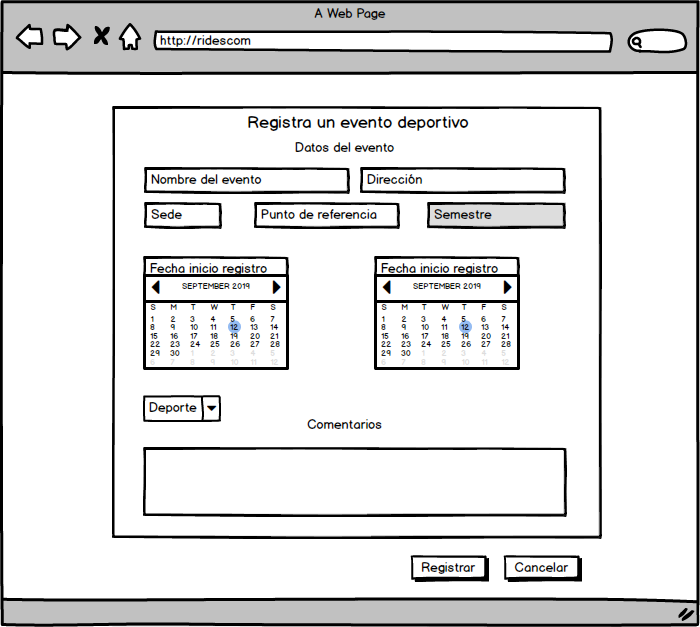
\includegraphics[width=10cm, height=6cm]{Imagenes/Nuevos/P4_Crear_evento_deportivo}
			\caption{Vista para dar de alta un evento deportivo (Jefe de Fomento Deportivo).}
			\label{creaevento}
		\end{figure}
		\pagebreak	
		
		\begin{figure} [hbt!]
			\centering
			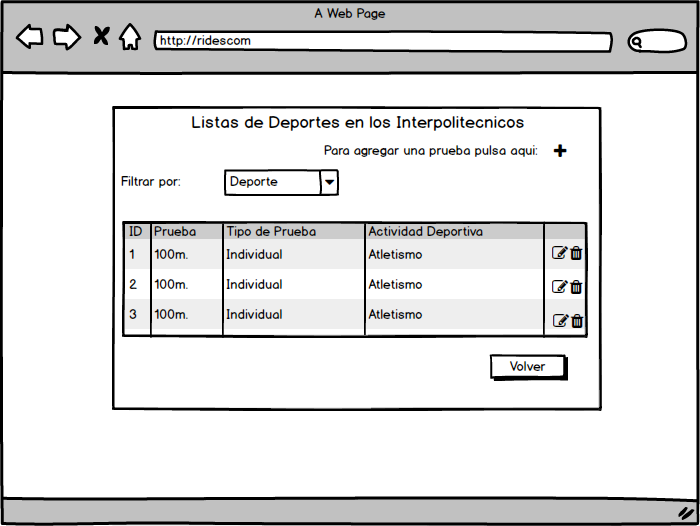
\includegraphics[width=10cm, height=6cm]{Imagenes/Nuevos/P27_Deportes_JFD}
			\caption{Página para visualizar los deportes que se llevaran a cabo en los eventos interpolitécnicos}
			\label{deportes}
		\end{figure}
	
		\begin{figure} [hbt!]
			\centering
			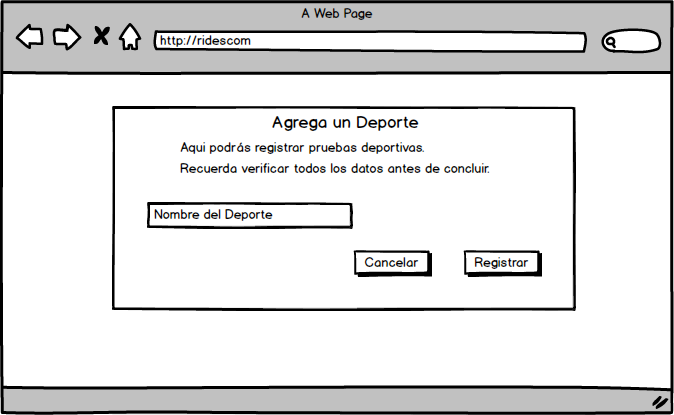
\includegraphics[width=10cm, height=6cm]{Imagenes/Nuevos/P28_AgregarDeportes_JFD}
			\caption{Página para agregar un deporte.}
			\label{agregadeporte}
		\end{figure}
		
		\begin{figure} [hbt!]
			\centering
			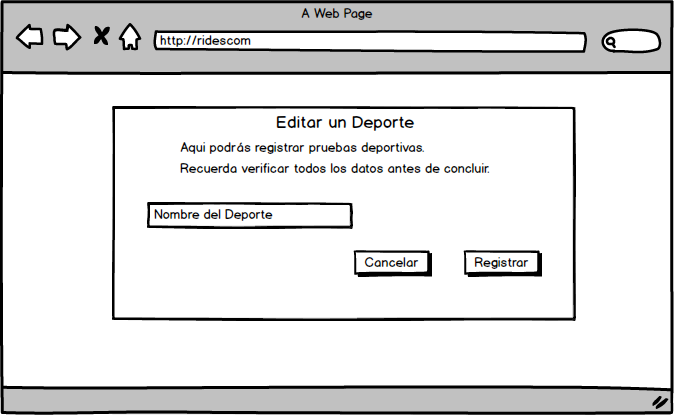
\includegraphics[width=10cm, height=6cm]{Imagenes/Nuevos/P29_EditarDeportes_JFD}
			\caption{Página para editar datos de los deportes}
			\label{editardeporte}
		\end{figure}
		\pagebreak
		
		\begin{figure} [hbt!]
			\centering
			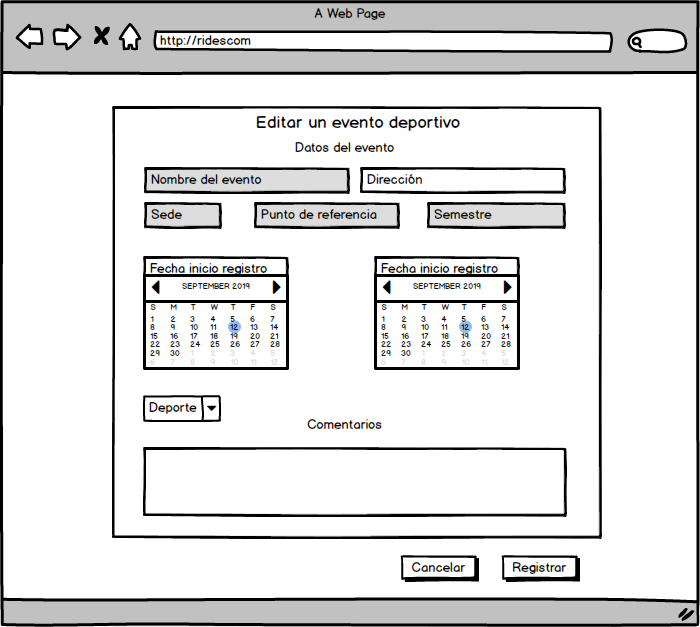
\includegraphics[width=10cm, height=6cm]{Imagenes/Nuevos/P5_Editar_evento_deportivo}
			\caption{Vista para editar datos de un evento ya registrado. (Jefe de FOmento Deportivo).}
			\label{editarevento}
		\end{figure}
	
		\begin{figure} [hbt!]
			\centering
			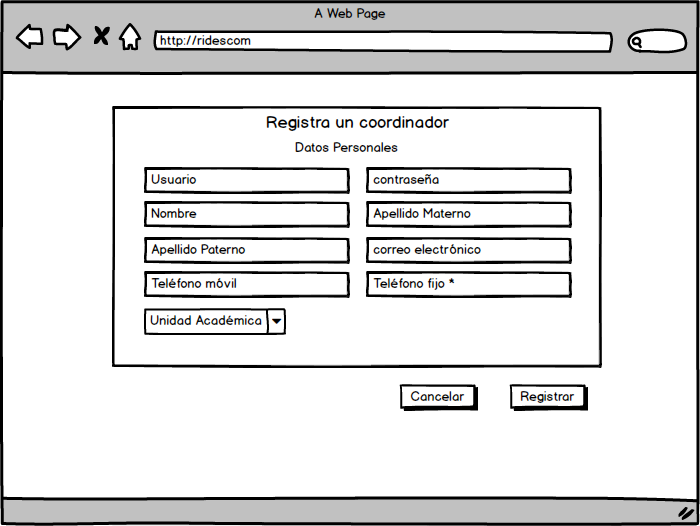
\includegraphics[width=10cm, height=6cm]{Imagenes/Nuevos/P6_Registro_coordinador}
			\caption{Vista para registrar un coordinador de unidad académica. (Jefe de Fomento Deportivo).}
			\label{registrarcoord}
		\end{figure}
		
		\begin{figure} [hbt!]
			\centering
			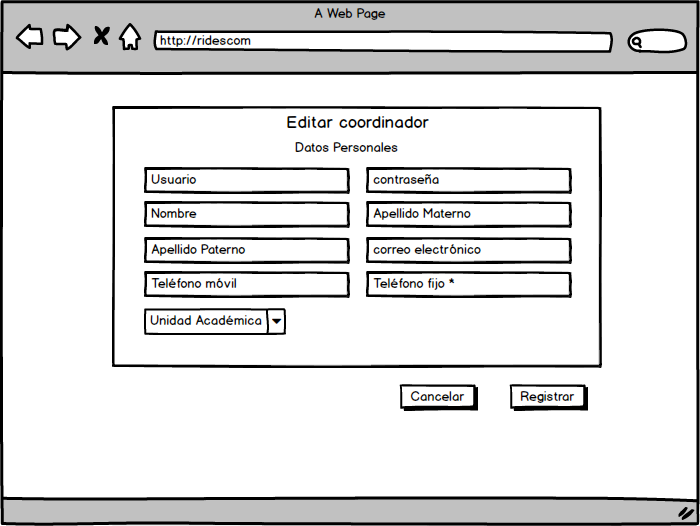
\includegraphics[width=10cm, height=6cm]{Imagenes/Nuevos/P7_Editar_coordinador}
			\caption{Vista para editar datos de un coordinador previamente registrado. (Jefe de Fomento Deportivo).}
			\label{editarcoord}
		\end{figure}
\pagebreak

		\begin{figure} [hbt!]
			\centering
			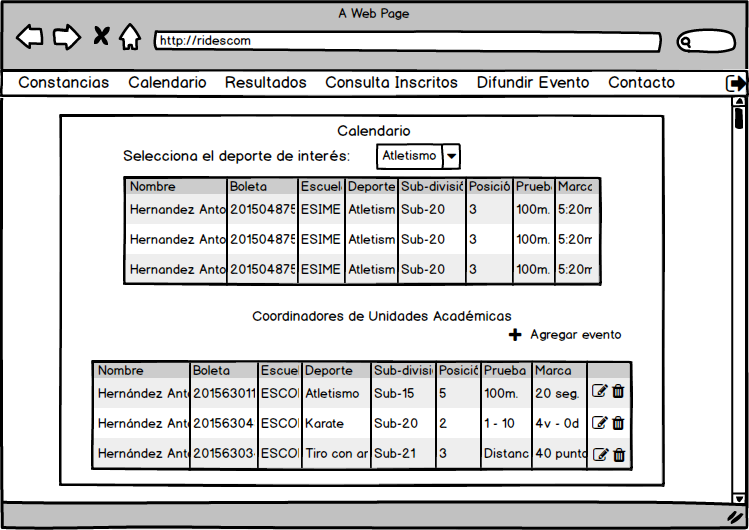
\includegraphics[width=10cm, height=6cm]{Imagenes/Nuevos/P8_Inicio_CoordUA}
			\caption{Vista principal para el coordinador de una Unidad Académica.}
			\label{principalcoord}
		\end{figure}
	
		\begin{figure} [hbt!]
			\centering
			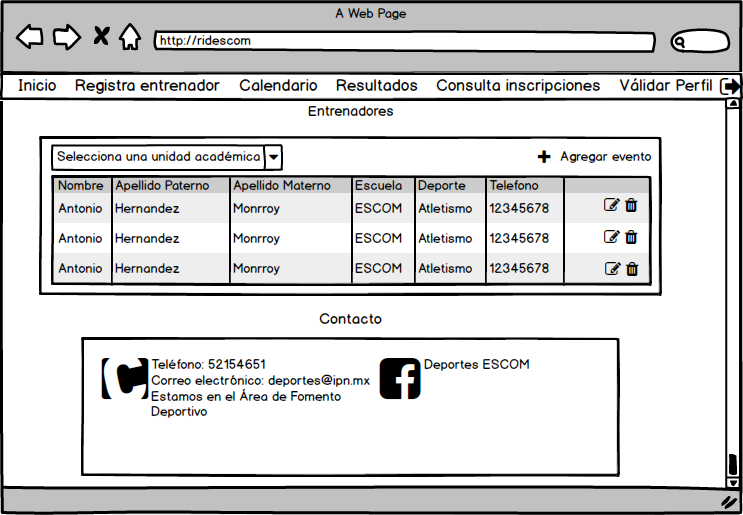
\includegraphics[width=10cm, height=6cm]{Imagenes/Nuevos/P9_Inicio_CoordUA1}
			\caption{Vista principal para el coordinador de una Unidad Académica (Continuación).}
			\label{principalcoord1}
		\end{figure}
	\pagebreak
		
		\begin{figure} [hbt!] 
			\centering
			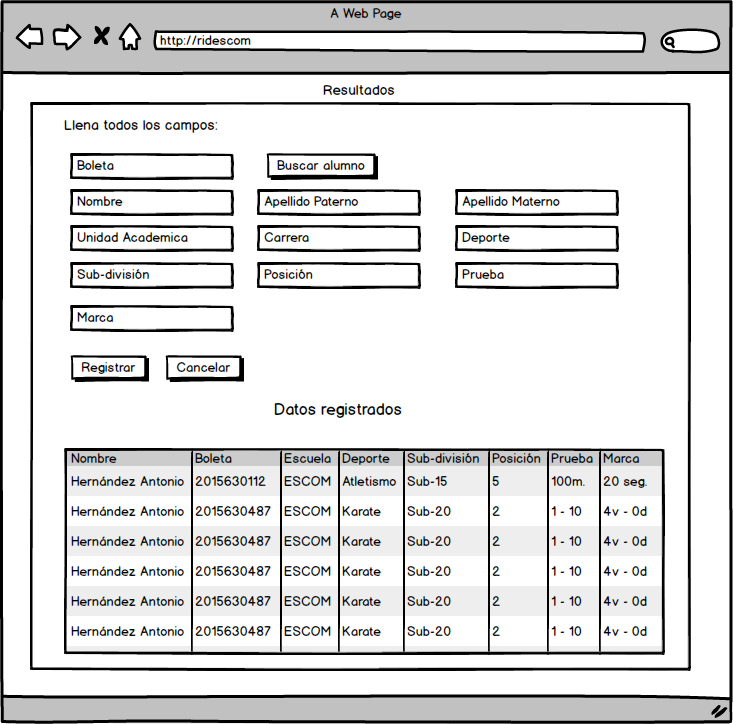
\includegraphics[width=10cm, height=7cm]{Imagenes/Nuevos/P10_Ingresa_resultados}
			\caption{Vista para ingresar los resultados obtenidos por los participantes (Coordinador de Unidad Académica).}
			\label{ingresaresultados}
		\end{figure}
		
		\begin{figure} [hbt!]
			\centering
			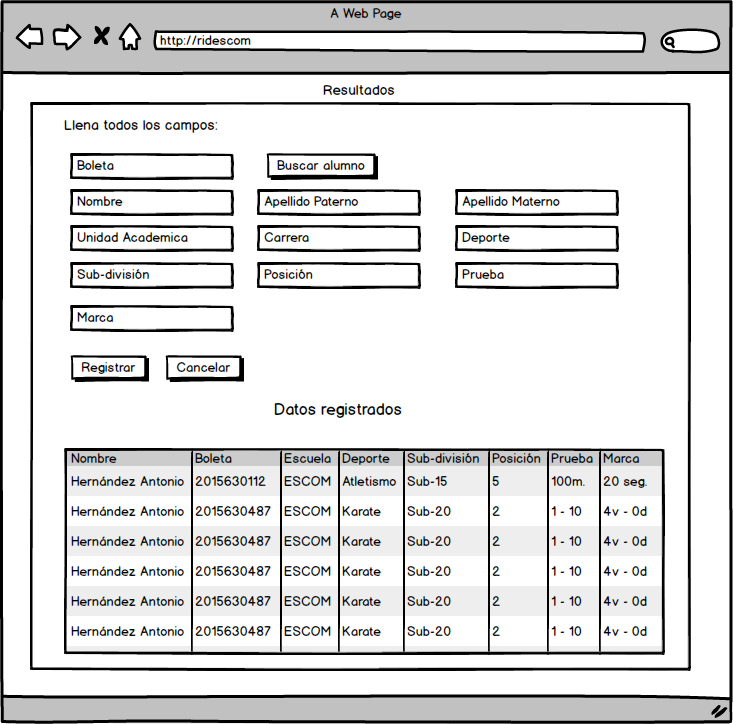
\includegraphics[width=10cm, height=7cm]{Imagenes/Nuevos/P11_Editar_resultados}
			\caption{Vista para editar los resultados de los participantes (Coordinador de Unidad Académica).}
			\label{editaresultados}
		\end{figure}
		\pagebreak
		
		\begin{figure} [hbt!]
			\centering
			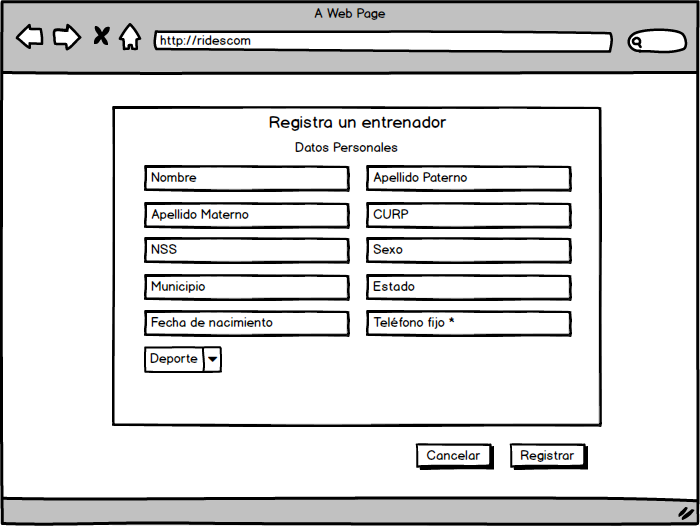
\includegraphics[width=10cm, height=6cm]{Imagenes/Nuevos/P12_Registro_entrenador}
			\caption{Vista para registrar a un entrenador (Coordinador de Unidad Académica).}
			\label{registroentrenador}
		\end{figure}
		
		\begin{figure} [hbt!]
			\centering
			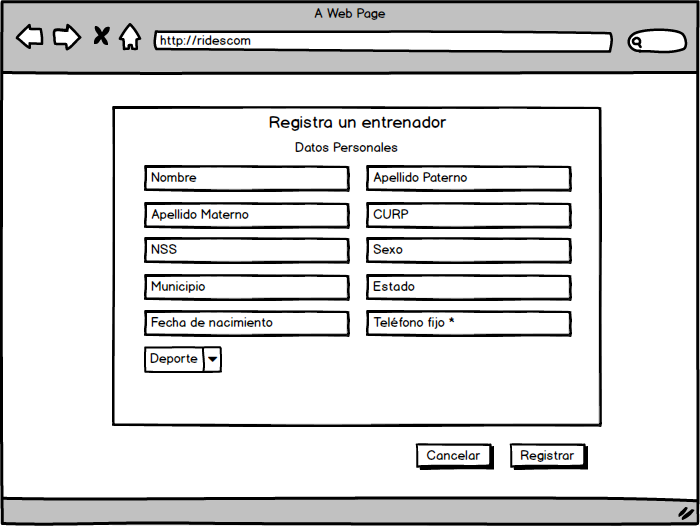
\includegraphics[width=10cm, height=6cm]{Imagenes/Nuevos/P13_Editar_entrenador}
			\caption{Vista para editar los datos del entrenador (Coordinador de Unidad Académica).}
			\label{editarentrenador}
		\end{figure}
		
		\begin{figure} [hbt!]
			\centering
			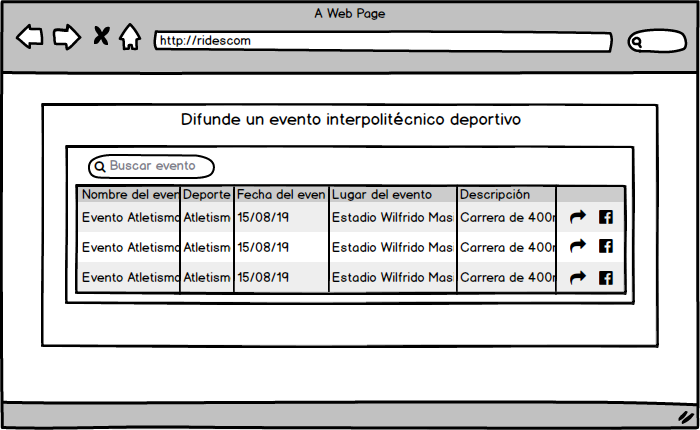
\includegraphics[width=10cm, height=6cm]{Imagenes/Nuevos/P14_Difundir_evento}
			\caption{Vista para difundir un evento interpolitécnico deportivo (Coordinador de Unidad Académica).}
			\label{difundirevento}
		\end{figure}
		\pagebreak

		\begin{figure} [hbt!]
			\centering
			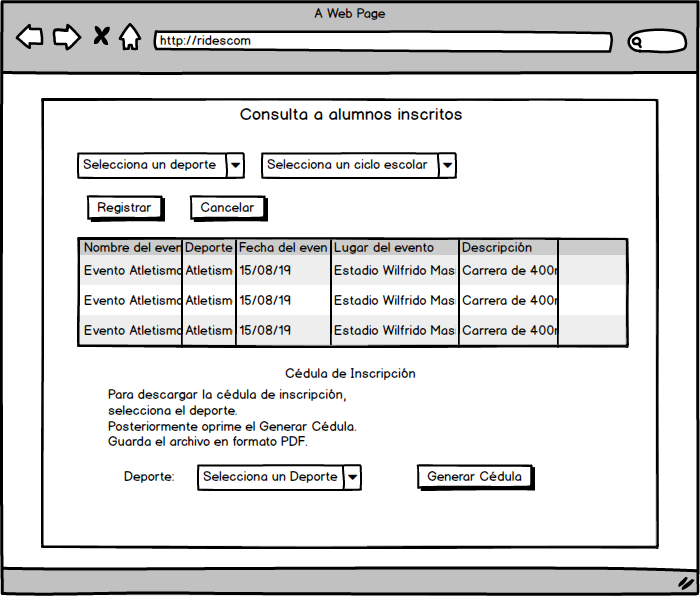
\includegraphics[width=10cm, height=6cm]{Imagenes/Nuevos/P15_Consulta_alumnos_inscritos}
			\caption{Vista para consultar los alumnos que se han inscrito a un evento (Coordinador de Unidad Académica).}
			\label{consultaalumnosinscritos}
		\end{figure}
	
		\begin{figure} [hbt!]
			\centering
			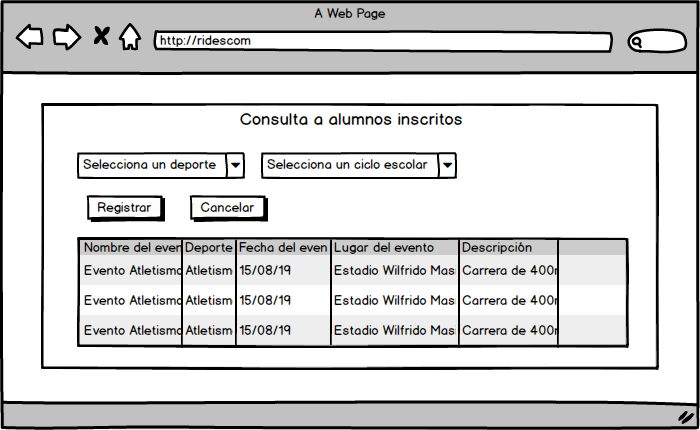
\includegraphics[width=10cm, height=6cm]{Imagenes/Nuevos/P16_Consulta_para_expedir_constancias}
			\caption{Vista para consultar participación de alumnos (Coordinador).}
			\label{consultaparaexpedirconstancias}
		\end{figure}
		
		\begin{figure} [hbt!]
			\centering
			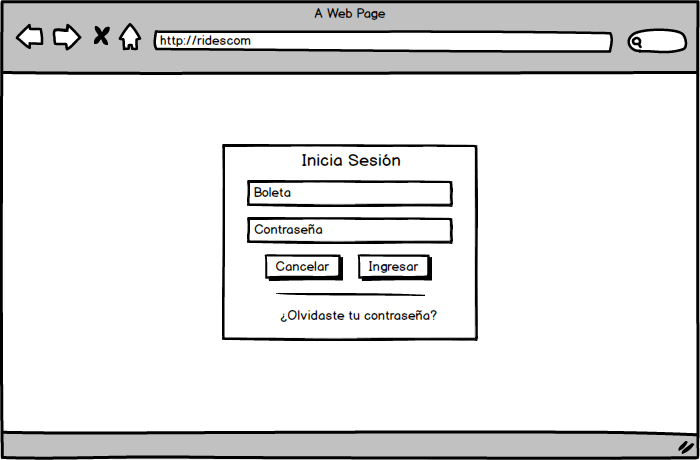
\includegraphics[width=10cm, height=6cm]{Imagenes/Nuevos/P17_Login_alumno}
			\caption{Vista Inicio de Sesión para el alumno.}
			\label{loginalumno}
		\end{figure}
	\pagebreak
		
		\begin{figure} [hbt!]
			\centering
			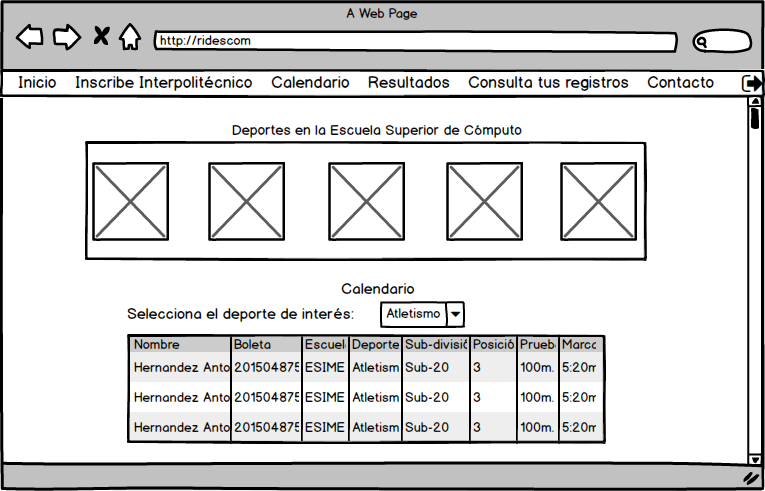
\includegraphics[width=10cm, height=6cm]{Imagenes/Nuevos/P18_Inicio_paticipante}
			\caption{Vista principal del alumno.}
			\label{principalalum}
		\end{figure}
		
		\begin{figure} [hbt!]
			\centering
			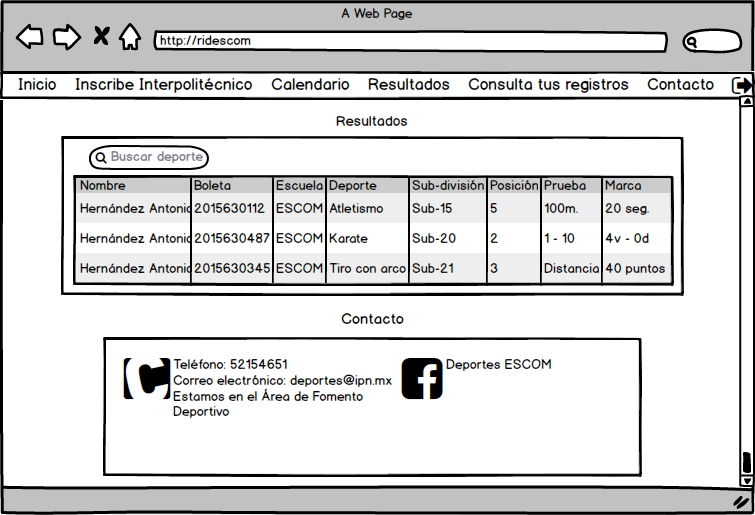
\includegraphics[width=10cm, height=6cm]{Imagenes/Nuevos/P19_Inicio_paticipante1}
			\caption{Vista principal del alumno (Continuación).}
			\label{principalalum1}
		\end{figure}
	
		\begin{figure} [hbt!]
			\centering
			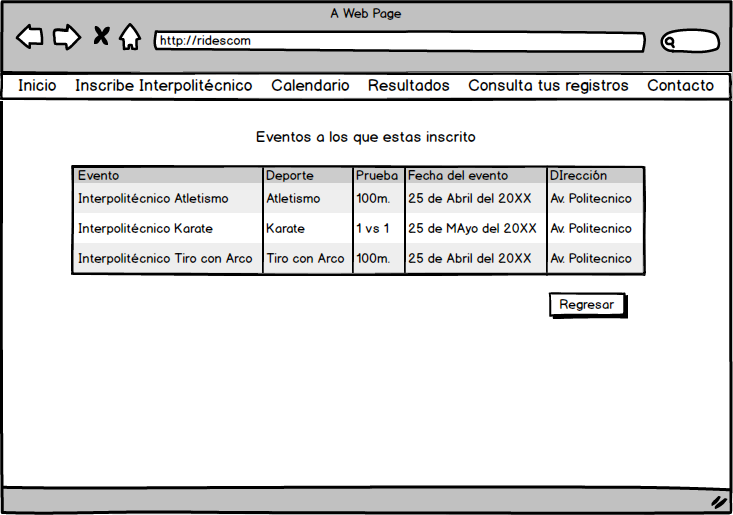
\includegraphics[width=10cm, height=6cm]{Imagenes/Nuevos/P20_Consulta_Inscripciones}
			\caption{Vista para consultar los eventos a los que se a registrado el alumno (Alumno).}
			\label{consultainscripcion}
		\end{figure}
	\pagebreak
		
		\begin{figure} [hbt!]
			\centering
			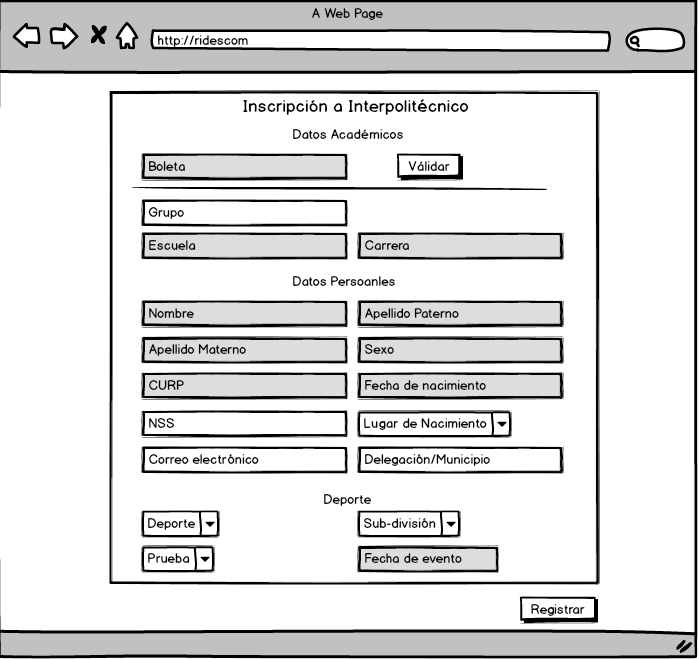
\includegraphics[width=10cm, height=6cm]{Imagenes/Disenos/Inscripcioninter}
			\caption{Formulario para que el alumno se registre en un evento interpolitécnico deportivo.}
			\label{Inscripcioninterpolitecnico}
		\end{figure}
		

		\begin{figure} [hbt!]
			\centering
			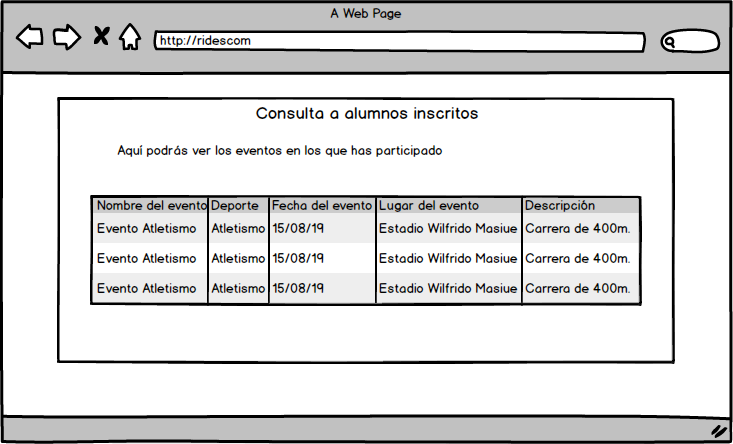
\includegraphics[width=10cm, height=6cm]{Imagenes/Nuevos/P21_Historial}
			\caption{Vista para que el alumno pueda visualizar todos los eventos en los que ha participado.}
			\label{historial}
		\end{figure}

	\chapter{Apartado D: Diagrama de Procesos}	
		\noindent Este apartado esta destinado para mostrar el diagrama del proceso actual refiriendose al proceso de inscripción a un evento interpolitécnico deportivo y a su vez, se muestra el proceso propuesto del mismo.
		
		\begin{figure}[hbt!]
			\centering
			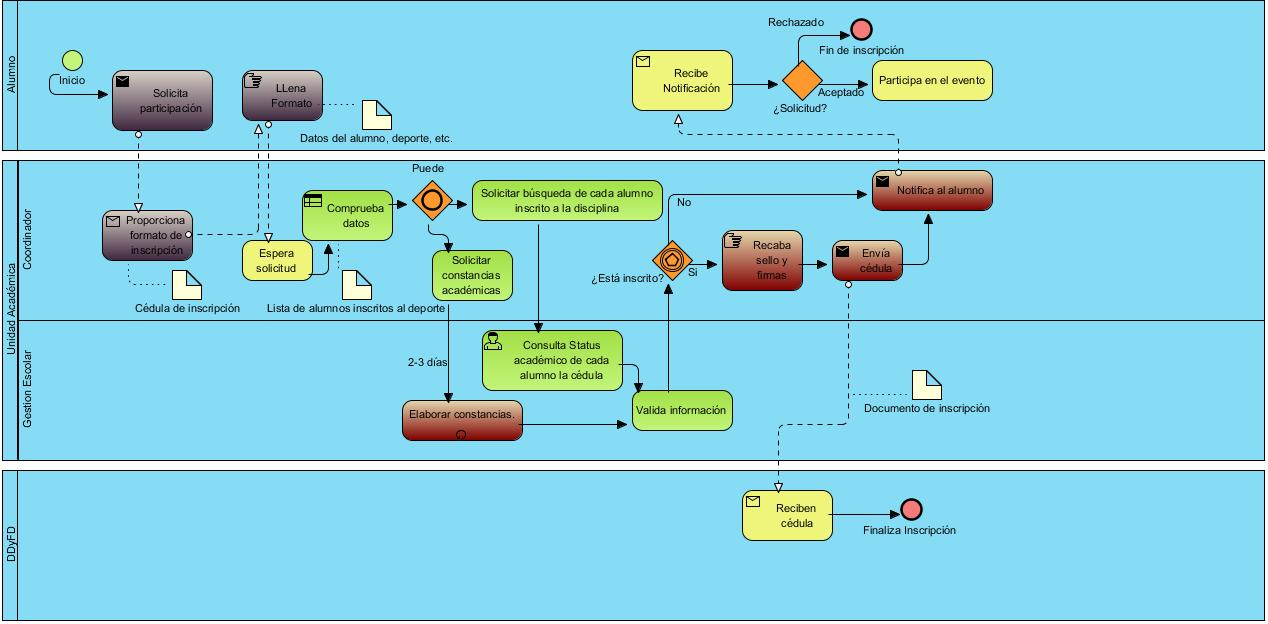
\includegraphics[width=16cm, height=8cm]{Imagenes/Disenos/ProcesoInscripcionActual.jpg}
			\caption{Proceso actual para la inscripcion a un evento interpolitécnico deportivo.}
			\label{ProcesoInscripcionActual}
		\end{figure}
	\pagebreak
	
		\begin{figure}[hbt!]
			\centering
			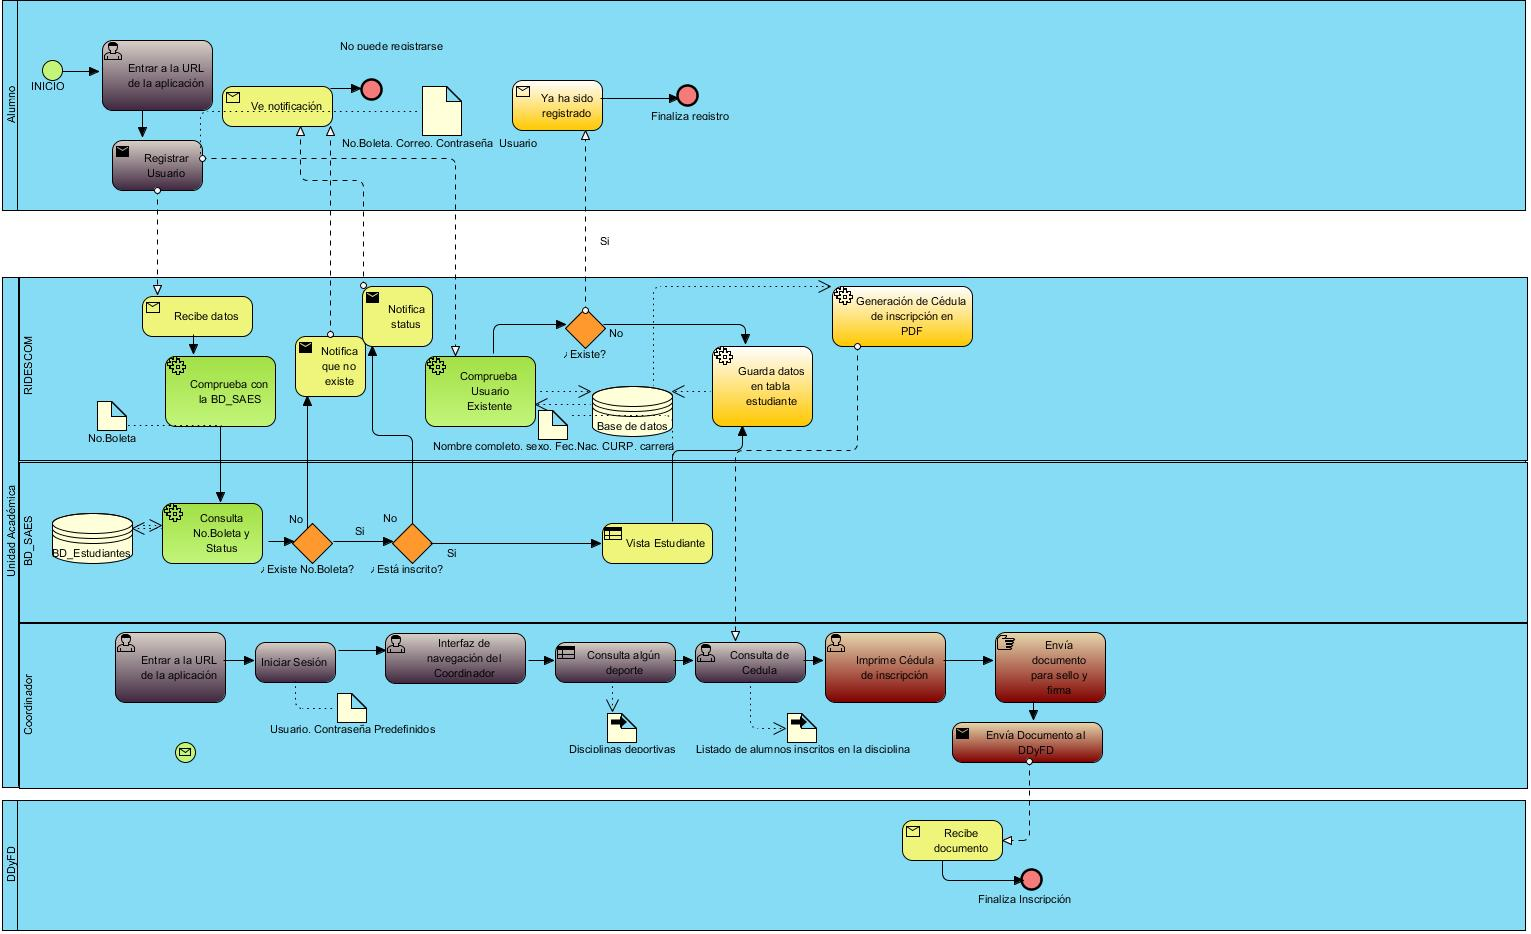
\includegraphics[width=16cm, height=8cm]{Imagenes/Disenos/ProcesoInscripcionPropuesto.jpg}
			\caption{Proceso propuesto para la inscripcion a un evento interpolitécnico deportivo.}
			\label{ProcesoInscripcionPropuesto}
		\end{figure}
	
	
	\chapter{Apartado E: Diagramas de Casos de Uso}
	\noindent En este apartado se muestra el diagrama de casos de uso de los actores, la interacción con cada uno de ellos y como funcionaria dentro de la aplicación web.
		\begin{figure}[hbt!]
			\centering
			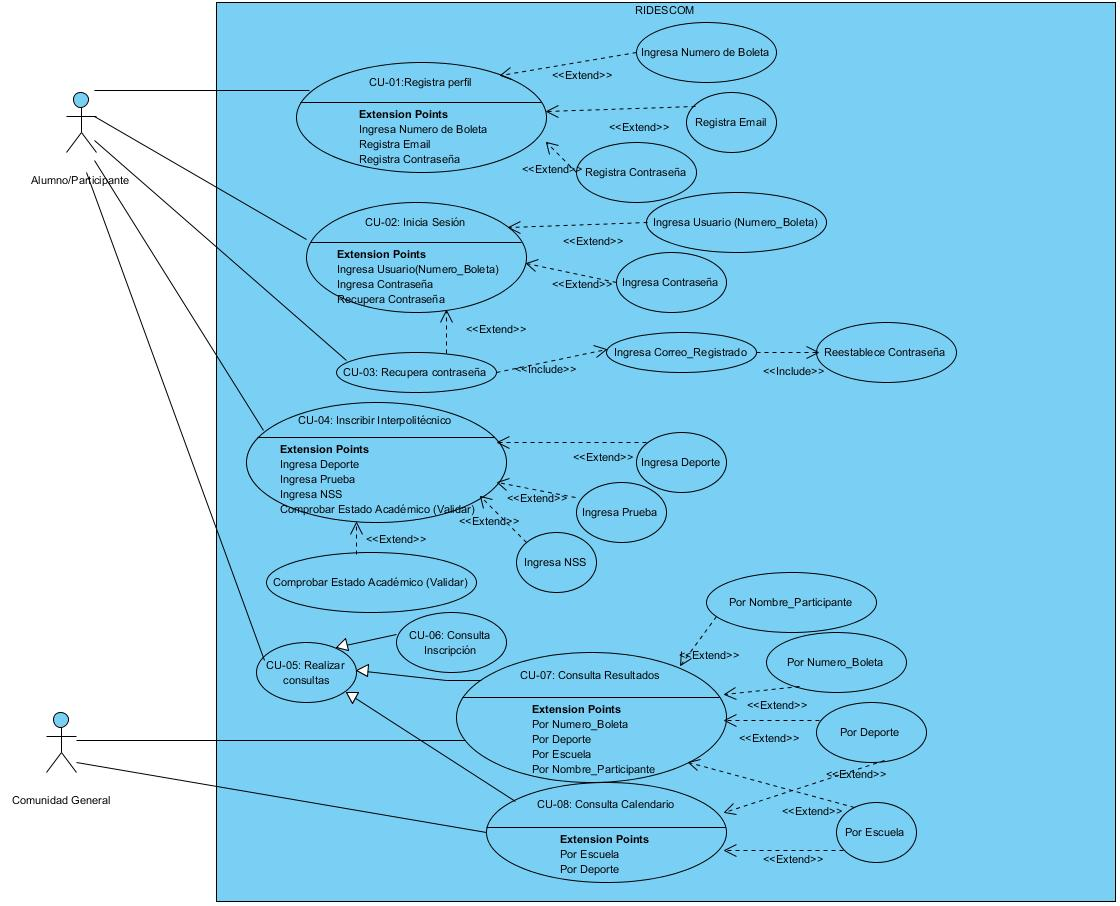
\includegraphics[width=16cm, height=8cm]{Imagenes/Disenos/DiagramasCU/Alumno.jpg}
			\caption{Diagrama de procesos Inscripción actual para un evento interpolitécnico deportivo.}
			\label{Inscripcion}
		\end{figure}
	\pagebreak
		\begin{figure}[hbt!]
			\centering
			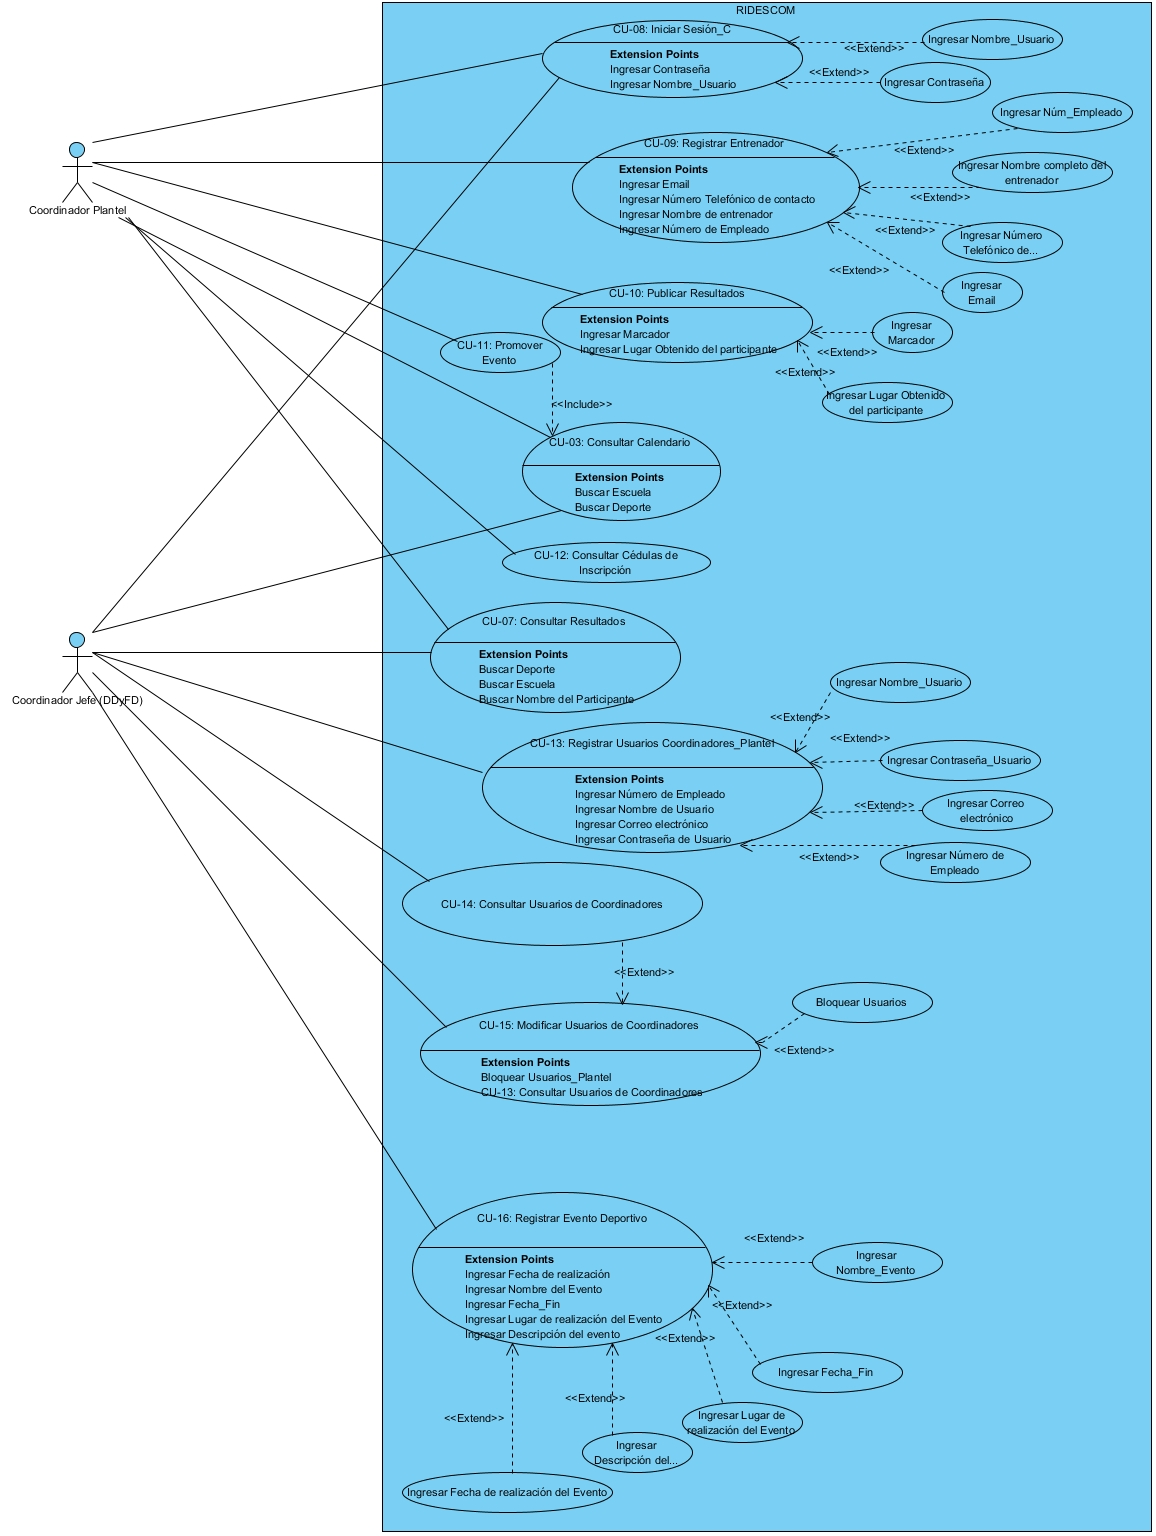
\includegraphics[width=16cm, height=12cm]{Imagenes/Disenos/DiagramasCU/CoordinadoresFinal.jpg}
			\caption{Diagrama de procesos Inscripción propuesto para un evento interpolitécnico deportivo.}
			\label{Inscripcion}
		\end{figure}
	
	\chapter{Apartado F: Crawler}
		\label{crawler}
		\noindent Este código fue desarrollado con el lenguaje de programación JAVA y JSOUP, permitiendo la simulación de la interacción de una persona “navegando” en la red, este “web crawler” fue desarrollado con el propósito de encontrar un mecanismo de validación para comprobar si realmente eres alumno de la ESCOM, donde se iniciará sesión con los datos del usuario de la plataforma de la escuela llamado SAES pidiendo un usuario (Boleta del alumno), contraseña y una clave captcha que el servidor de la plataforma genera como un filtro para evitar la intrusión de “bots informáticos”.\\
		
		\begin{figure}[hbt!]
			\centering
			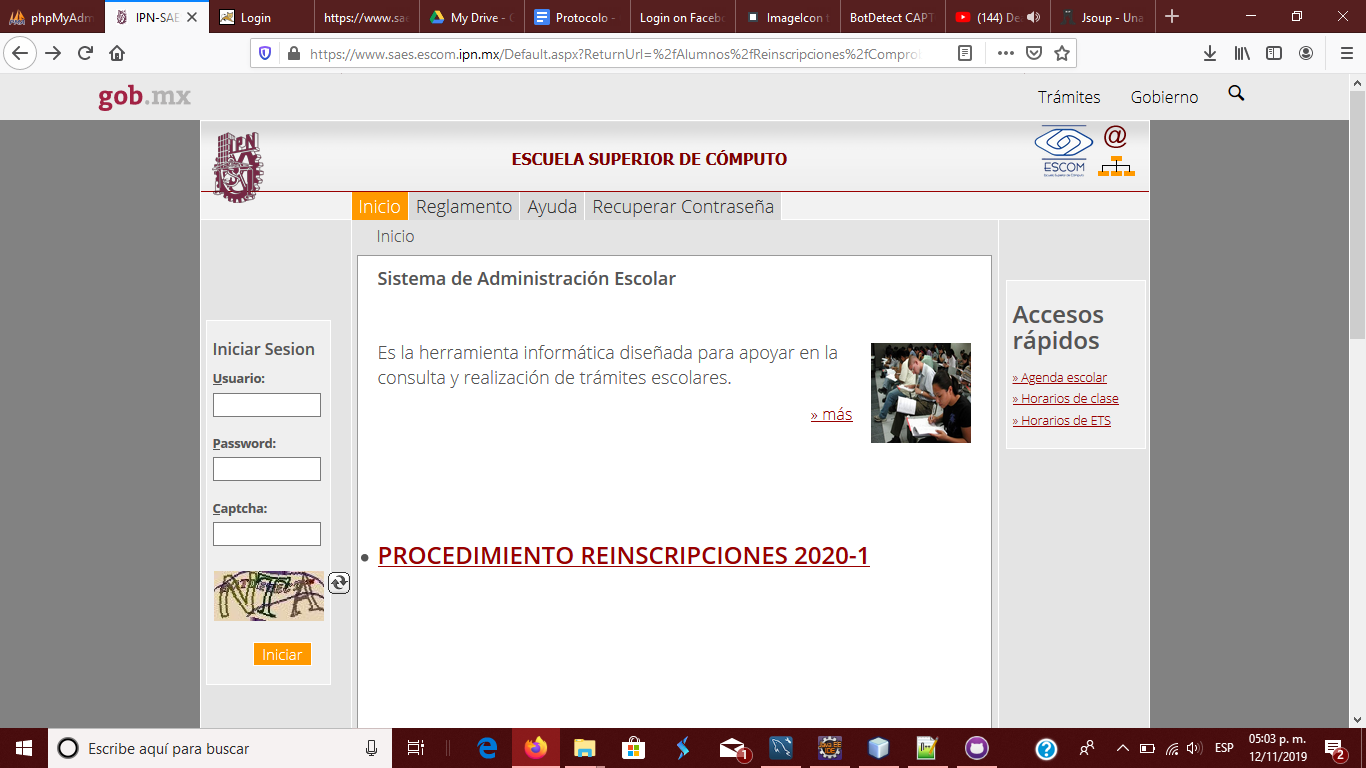
\includegraphics[width=10cm, height=6cm]{Imagenes/Crawler/SAES}
			\caption{Página del SAES Escom}
			\label{saes}
		\end{figure}
	
		\noindent Mediante las herramientas como JSOUP nos permite obtener información del HTML de cualquier página en la web, a excepción de la información generada con javascript pues las obtenciones de información son extraídas de manera estática y no de forma dinámica, o bien desde la lectura del HTML.\\
		\noindent Las pruebas de este código fueron realizadas durante los meses de enero del 2019 y octubre del mismo año. Utilizando así el siguiente código.
\pagebreak
		
		\noindent Por inicio tenemos que importar las librerías de JSOUP para hacer uso de los métodos que se presentarán a continuación, además de crear datos públicos para los métodos de las clases java para utilizarlos posteriormente.\\
		\noindent Creamos la conexión con la página que queremos explorar y solicitar una respuesta de esta conexión realizada junto con las “cookies” generadas en esta respuesta, ya que estás nos darán pauta para mantenernos en la misma conexión con respecto a la solicitud de conexión hecha anteriormente. \\
		
		\begin{figure} [hbt!]
			\centering
			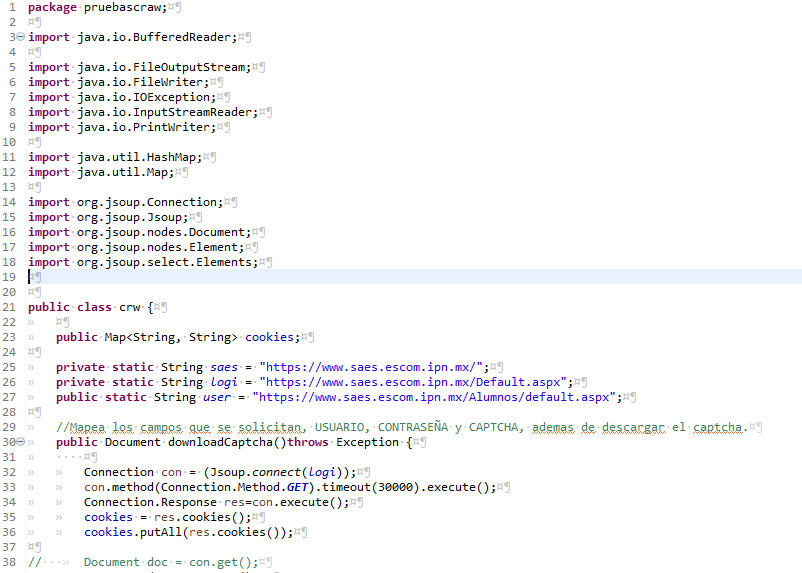
\includegraphics[width=10cm, height=6cm]{Imagenes/Crawler/Codigo1}
			\caption{Código desarrollado implementando el crawler.}
			\label{codigo1}
		\end{figure}
		
		\noindent Lo siguiente es realizar la exploración de los elementos del HTML en una variable de tipo “Document” de la página solicitada donde buscaremos el elemento por ID del CAPTCHA del HTML y así crear una imagen válida que fuese creada por el servidor, extrayendo la ubicación de la imagen para colocarla en una respuesta de conexión con la ruta de la imagen obtenida en la variable “a” y generarla de manera local utilizando “FileOutputStream”, el método creado es de tipo “Document” por lo tanto su salida es del mismo tipo. 
\pagebreak
		
		\begin{figure} [hbt!]
			\centering
			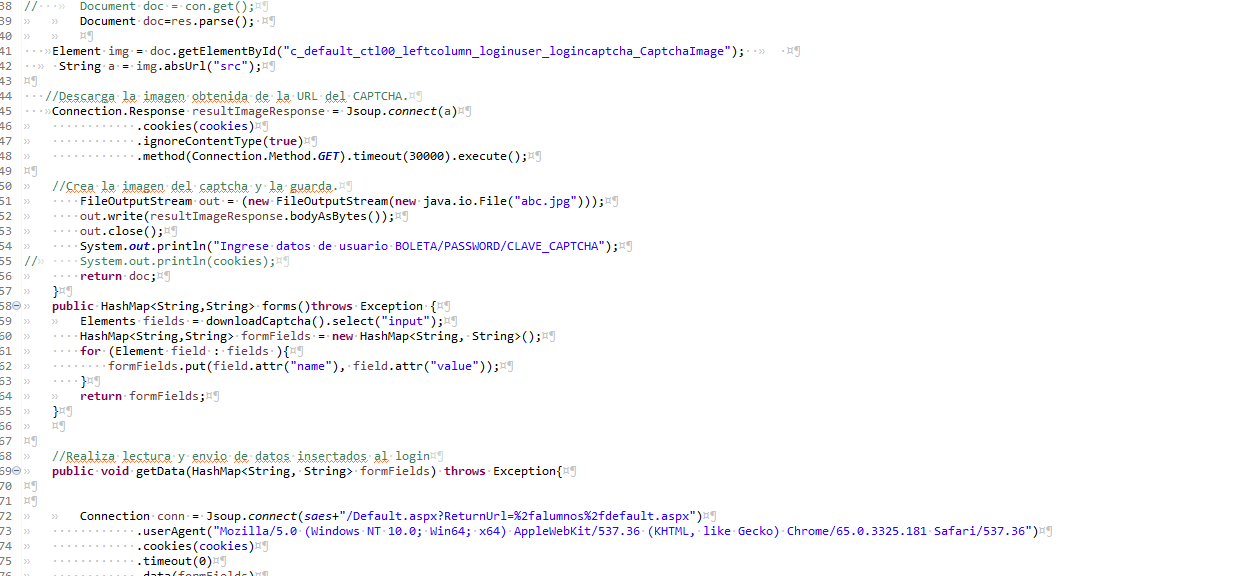
\includegraphics[width=10cm, height=8cm]{Imagenes/Crawler/Codigo2}
			\caption{Continuación de la implementación del crawler.}
			\label{codigo2}
		\end{figure}
		
		\noindent Una vez realizado este método procedemos a explorar los campos de inserción que existen en el HTML, para ello hacemos otra búsqueda de elementos en el HTML y definimos los datos que contienen estos elementos para su posterior inserción y uso de ellos mediante una variable de tipo “HashMap<String,String>” (todos los campos son de tipo cadena).\\
		
		\noindent Ahora la realización del método “getData(HashMap<String,String> formFields)” utilizaremos como parámetros los elementos de inserción explorados anteriormente insertándolos en nuestro método “POST”. Creamos la conexión a donde se debe redirigir la información del inicio de sesión, insertando también las cookies almacenadas en la previa conexión de la obtención del HTML de la página del SAES.\\
		
		\begin{figure} [hbt!]
			\centering
			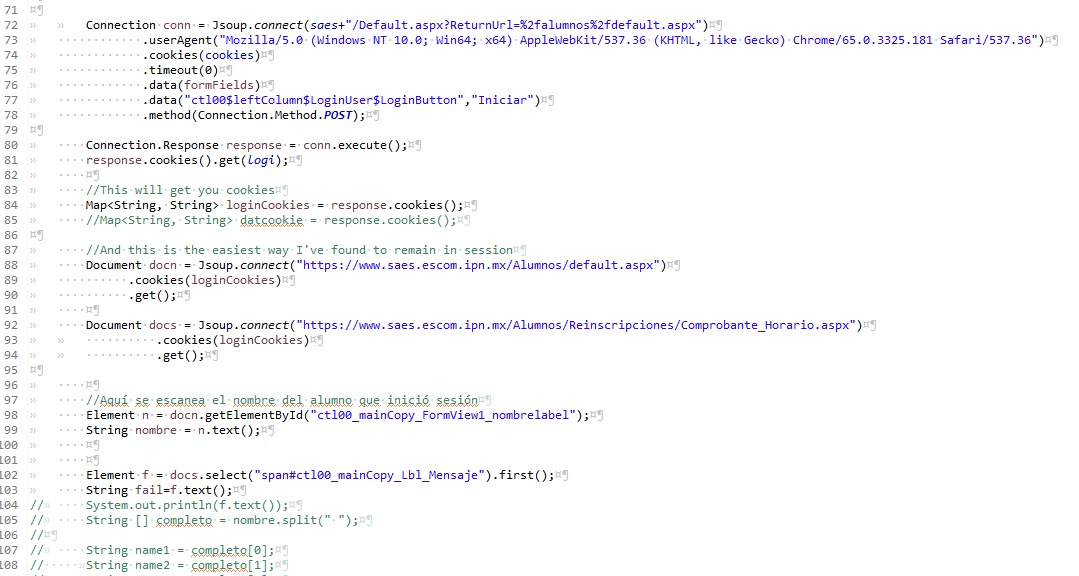
\includegraphics[width=10cm, height=8cm]{Imagenes/Crawler/Codigo3}
			\caption{Continuación implementación del crawler.}
			\label{codigo3}
		\end{figure}
	\pagebreak
	
	\noindent Si los datos ingresados son correctos se realizará una respuesta de la ruta solicitada en el POST insertando las cookies correspondientes a la conexión para comprobar la sesión del usuario en la plataforma, seguido de un mapeo del nuevo HTML donde se realizará la búsqueda por ID del campo donde se encuentre el nombre del alumno y un mensaje donde solo habrá texto si el usuario que haya iniciado sesión no estuviera inscrito.\\
	\noindent De lo anterior y siguiendo la condición de que el usuario que haya iniciado sesión esté o no inscrito dependerá si el texto buscado como “fail” sea nulo/vacío, en el caso de que no lo esté indicará que el alumno que haya iniciado sesión está “INSCRITO” indicando el nombre del alumno que corresponda a la boleta y usuario junto con un grupo al que pertenezca, en el caso de que “fail” no sea nulo/vacío se indicará que el alumno que corresponda a la boleta y usuario aparezca como “NO INSCRITO”. \\
	\begin{figure}[hbt!]
		\centering
		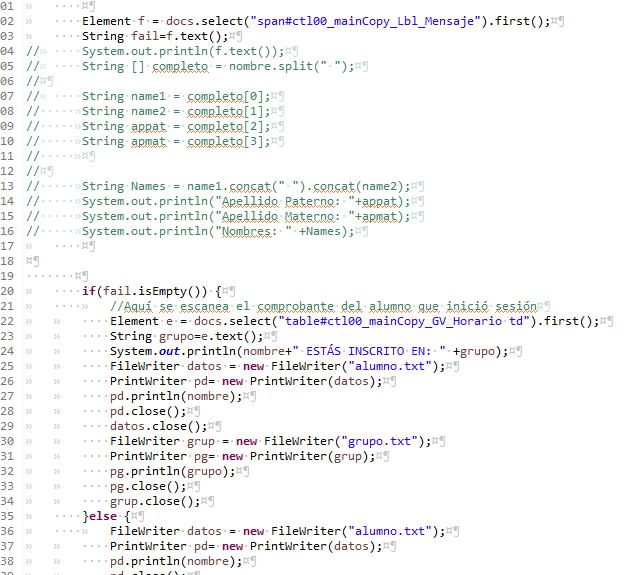
\includegraphics[width=10cm, height=8cm]{Imagenes/Crawler/Codigo4}
		\caption{Continuación implementación del crawler.}
		\label{codigo4}
	\end{figure}

	\noindent Finalmente se crean 3 archivos donde se almacena la información del usuario que haya iniciado sesión donde se inserta su nombre completo (alumno.txt), su grupo al que esté inscrito (grupo.txt) y el código HTML de la página donde se obtuvo toda esta información (respoinse.html).
\pagebreak

	\begin{figure}[hbt!]
		\centering
		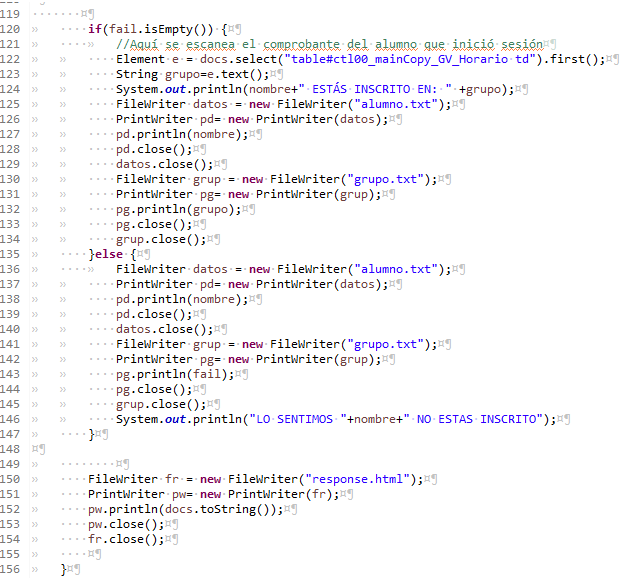
\includegraphics[width=10cm, height=6cm]{Imagenes/Crawler/Codigo5}
		\caption{Continuación de la implementación del crawler.}
		\label{codigo5}
	\end{figure}

	\noindent Una vez realizado esto necesitamos adjuntar estos métodos en 1 sola petición (o método) para realizar su ejecución e inserción de datos correspondientes a los que se necesitan.
	Como se hace en el método “run()”. \\
	
	\noindent Creamos un método donde se adjunta en 1 petición la ejecución de todos los métodos anteriores, y haremos la petición de los datos del inicio de sesión del SAES usando “readLine()” para hacer la lectura de estas seguido de la asignación de los campos que se escogen para insertar estas cadenas y reenviarlos al método “getData” donde los datos insertados serán los parámetros que servirán para la correcta funcionalidad del método “getData” y finalmente iniciar sesión.\\
	\begin{figure} [hbt!]
		\centering
		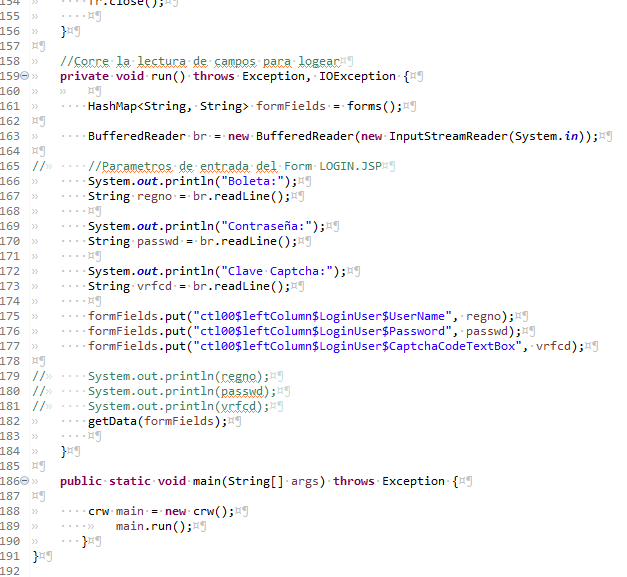
\includegraphics[width=10cm, height=8cm]{Imagenes/Crawler/Codigo6}
		\caption{Continuación implementación crawler.}
		\label{codigo6}
	\end{figure}
\pagebreak
	\noindent Cabe mencionar que dicha plataforma está desarrollada con ASP.NET con un plugin detector de “bots” llamado “Captcha BotDetect”, donde desde el servidor se realiza la generación de credenciales correspondientes a la imagen que se muestre en la página como la conocemos.\\
	\textbf{“href="BotDetectCaptcha.ashx?get=layoutStyleSheet" ”}\\
	\begin{figure} [hbt!]
		\centering
		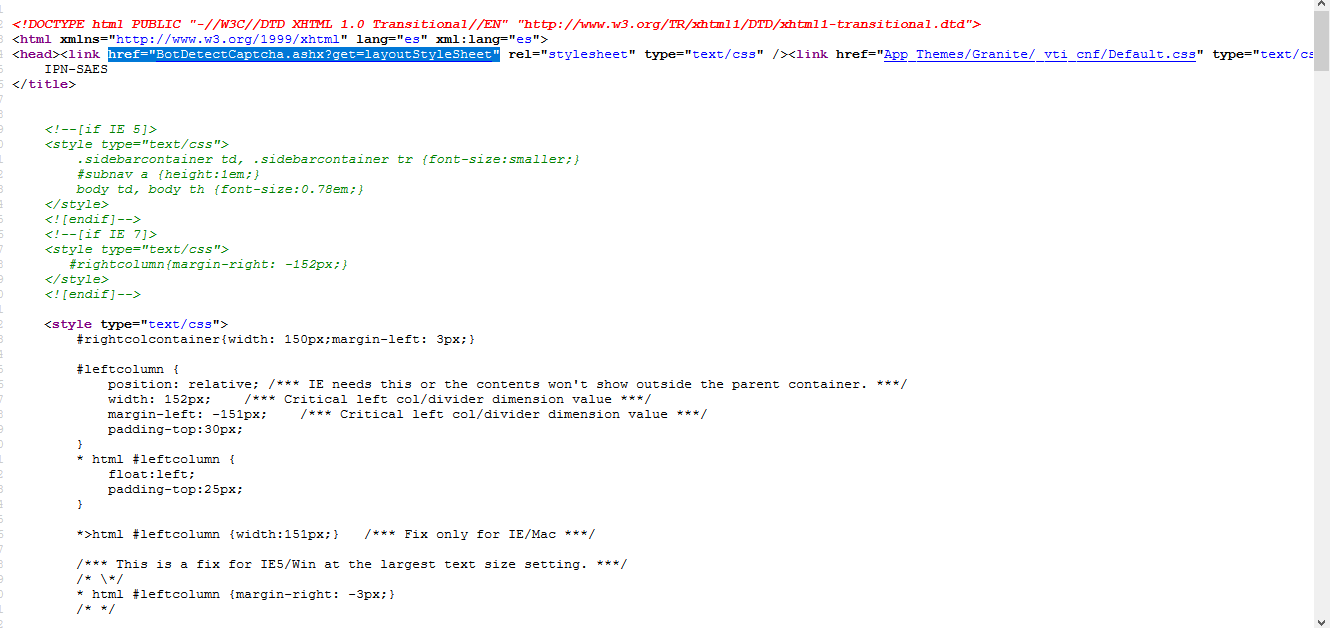
\includegraphics[width=10cm, height=6cm]{Imagenes/Crawler/ASP2}
		\caption{Inspección de estructura del SAES.}
		\label{asp2}
	\end{figure}

	\noindent Las peticiones de inicio de sesión se realizan directo al servidor y el servidor responde con un javascript donde redirecciona a la vista correspondiente si las credenciales de usuario y clave captcha son las correctas de acuerdo a la sesión de página en la que se encuentra.\\
	\textbf{“action="Default.aspx?ReturnUrl=\%2fAlumnos\%2fcambia\_clave.aspx" onsubmit="javascript:return WebForm\_OnSubmit();" ”}
	
	\begin{figure} [hbt!]
		\centering
		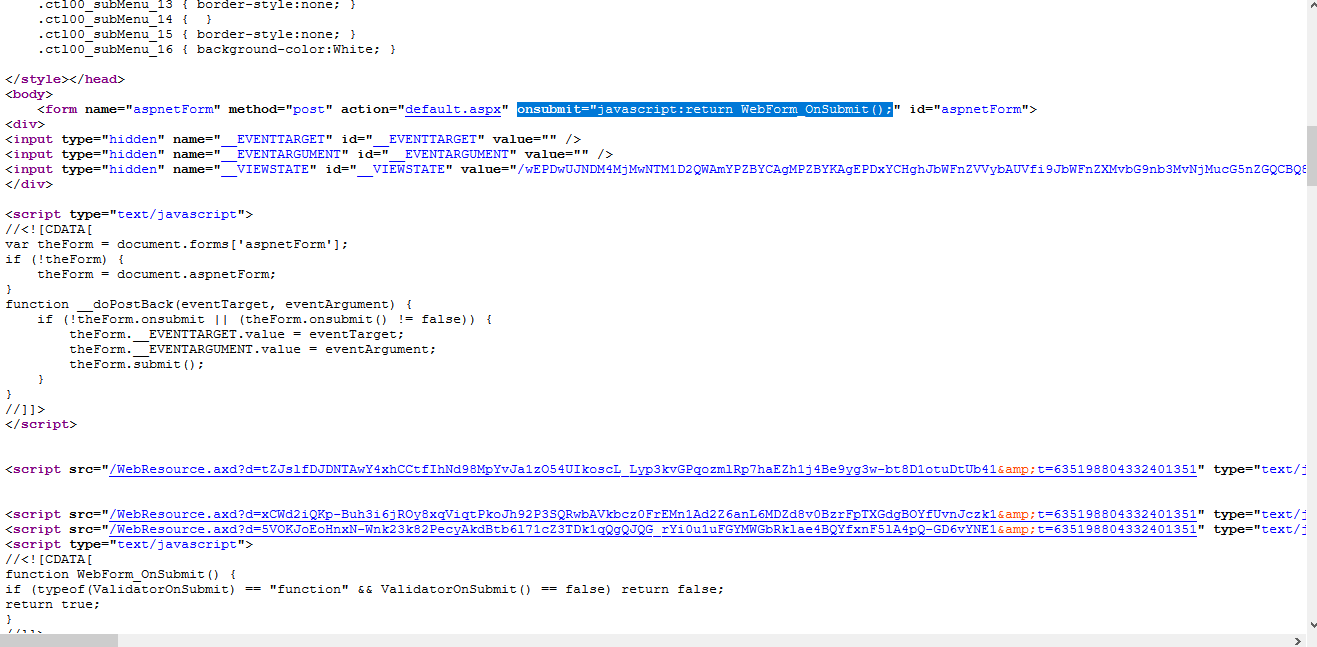
\includegraphics[width=10cm, height=6cm]{Imagenes/Crawler/ASP1}
		\caption{Inspección de estructura del SAES.}
		\label{asp1}
	\end{figure}
	\noindent Estos cambios se identificaron el día 15 de octubre del 2019.
\pagebreak
	
	\textbf{POR EJEMPLO: CON USUARIO NO INSCRITO}\\
	\noindent Se inserta previamente la boleta y contraseña del alumno del SAES ESCOM.
	
	\begin{figure}[hbt!]
		\centering
		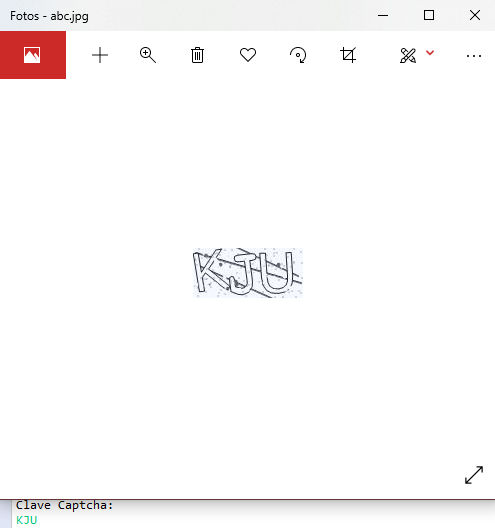
\includegraphics[width=10cm, height=5cm]{Imagenes/Crawler/ImagenloginNoinscrito}
		\caption{Captcha para alumno no inscrito.}
		\label{imagenloginnoinscrito}
	\end{figure}
	
	Se ingresa la clave captcha mostrada en la imagen “KJU”
	
	\begin{figure}[hbt!]
		\centering
		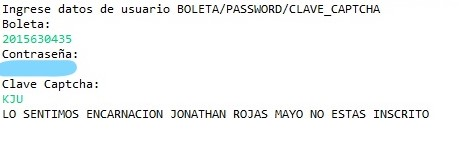
\includegraphics[width=10cm, height=5cm]{Imagenes/Crawler/Datosloginnoinscrito}
		\caption{Se ingresan los datos en el crawler.}
		\label{datosloginnoinscrito}
	\end{figure}
	\noindent Responde de acuerdo a la inscripción del alumno, para este caso el alumno NO ESTÁ INSCRITO.
\pagebreak

	\begin{figure}[hbt!]
		\centering
		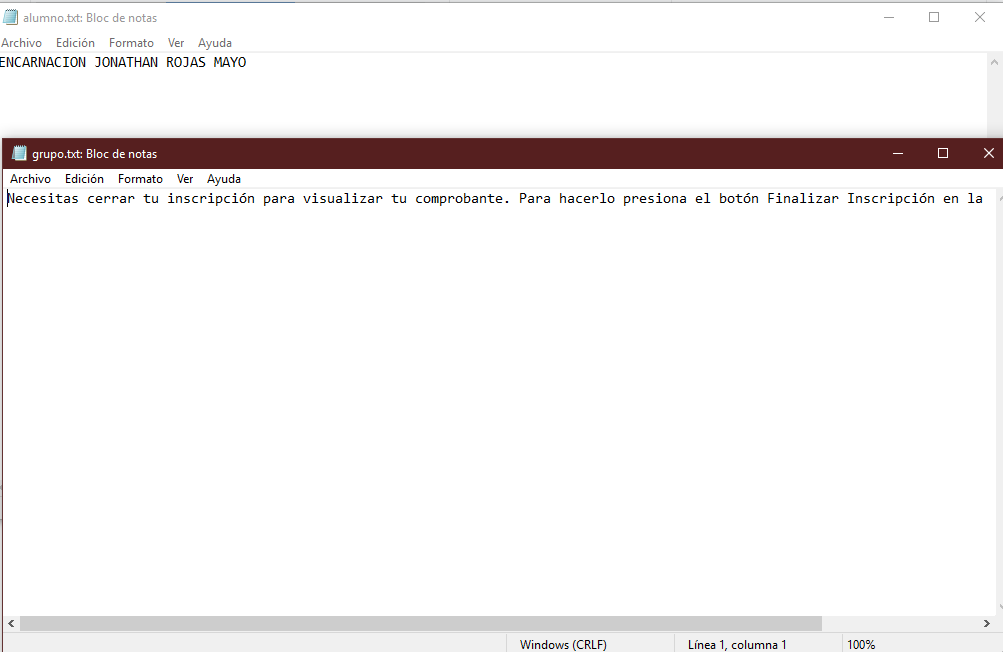
\includegraphics[width=10cm, height=6cm]{Imagenes/Crawler/Noinscrito}
		\caption{Respuesta del crawler.}
		\label{noinscrito}
	\end{figure}

	\noindent Se muestran las cadenas correspondientes a la extracción de información para validar que el alumno en cuestión esté inscrito o no lo esté.\\
	
	\textbf{POR EJEMPLO: CON USUARIO INSCRITO}\\
	\noindent Se inserta previamente la boleta y contraseña del alumno del SAES ESCOM.
	
	\begin{figure}[hbt!]
		\centering
		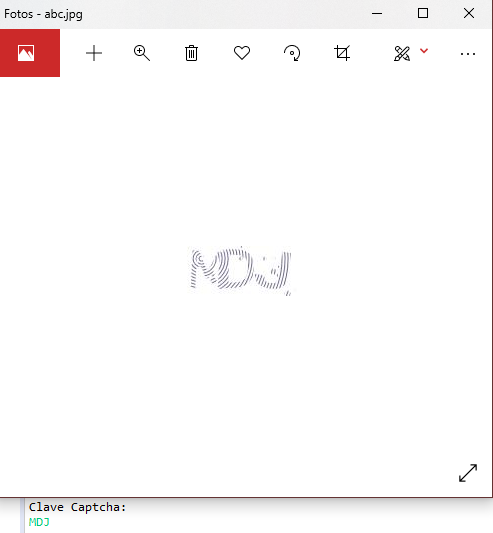
\includegraphics[width=10cm, height=6cm]{Imagenes/Crawler/Imagenlogininscrito}
		\caption{Captcha para el alumno inscrito.}
		\label{imagenlogininscrito}
	\end{figure}
	\noindent Se ingresa la clave captcha mostrada en la imagen “MDJ”
\pagebreak
	
	\begin{figure}[hbt!]
		\centering
		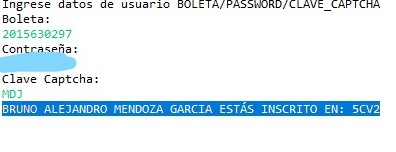
\includegraphics[width=10cm, height=6cm]{Imagenes/Crawler/Datoslogininscrito}
		\caption{Se registran ingresan datos al crawler.}
		\label{datoslogininscrito}
	\end{figure}
	
	\noindent Responde de acuerdo a la inscripción del alumno, para este caso el alumno ESTÁ INSCRITO.
	
	\begin{figure}[hbt!]
		\centering
		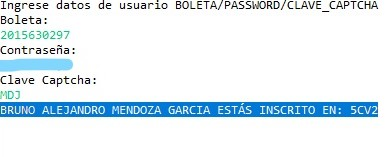
\includegraphics[width=10cm, height=6cm]{Imagenes/Crawler/Logininscrito}
		\caption{Respuesta del crawler.}
		\label{logininscrito}
	\end{figure}
	
	\begin{figure} [hbt!]
		\centering
		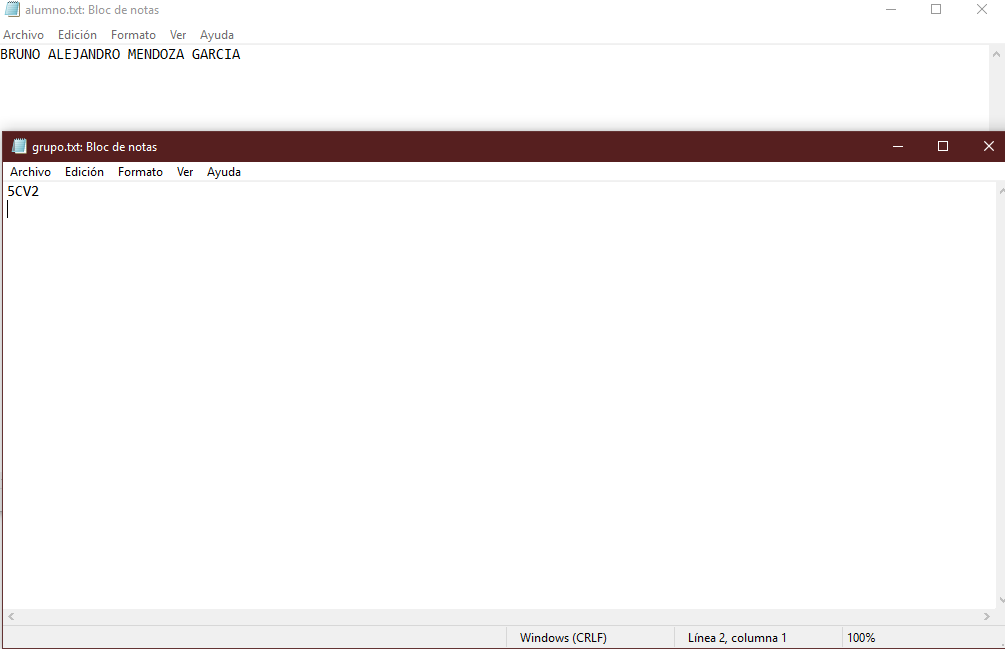
\includegraphics[width=10cm, height=6cm]{Imagenes/Crawler/Infologininscrito}
		\caption{Información del alumno inscrito.}
		\label{infologininscrito}
	\end{figure}
	\noindent Se muestran las cadenas correspondientes a la extracción de información para validar que el alumno en cuestión esté inscrito o no lo esté.

	\chapter{Apartado G: API Facebook}
	\label{apiFB}
	\noindent En este apartado, se menciona detalladamente la función e implementación al proyecto. Así como lo desarrollado y la problemática que se tuvo al final de la presentación del proyecto.\\
		
	Durante el periodo de pruebas realizado en Trabajo Terminal 2 nos percatamos que el módulo de difusión de eventos, no funcionaba de la manera correcta, por lo cual se realizó una revisión de este. Siendo así, nos percatamos que los terminos de uso de las herramientas de Facebook solicitaban una revisión de datos para que estás puedan ser empleadas en el proyecto, como se puede apreciar en la figura a continuación.
	
	Dentro de la investigacion se encontró que se  tenía que seguir paso a pasola verificación del negoncio y la revisión de la aplicación, con la finalidad de si está todo en orden se pueda utilizar las herramientas de Facebook.
	
	\begin{figure}[hbt!]
		\centering
		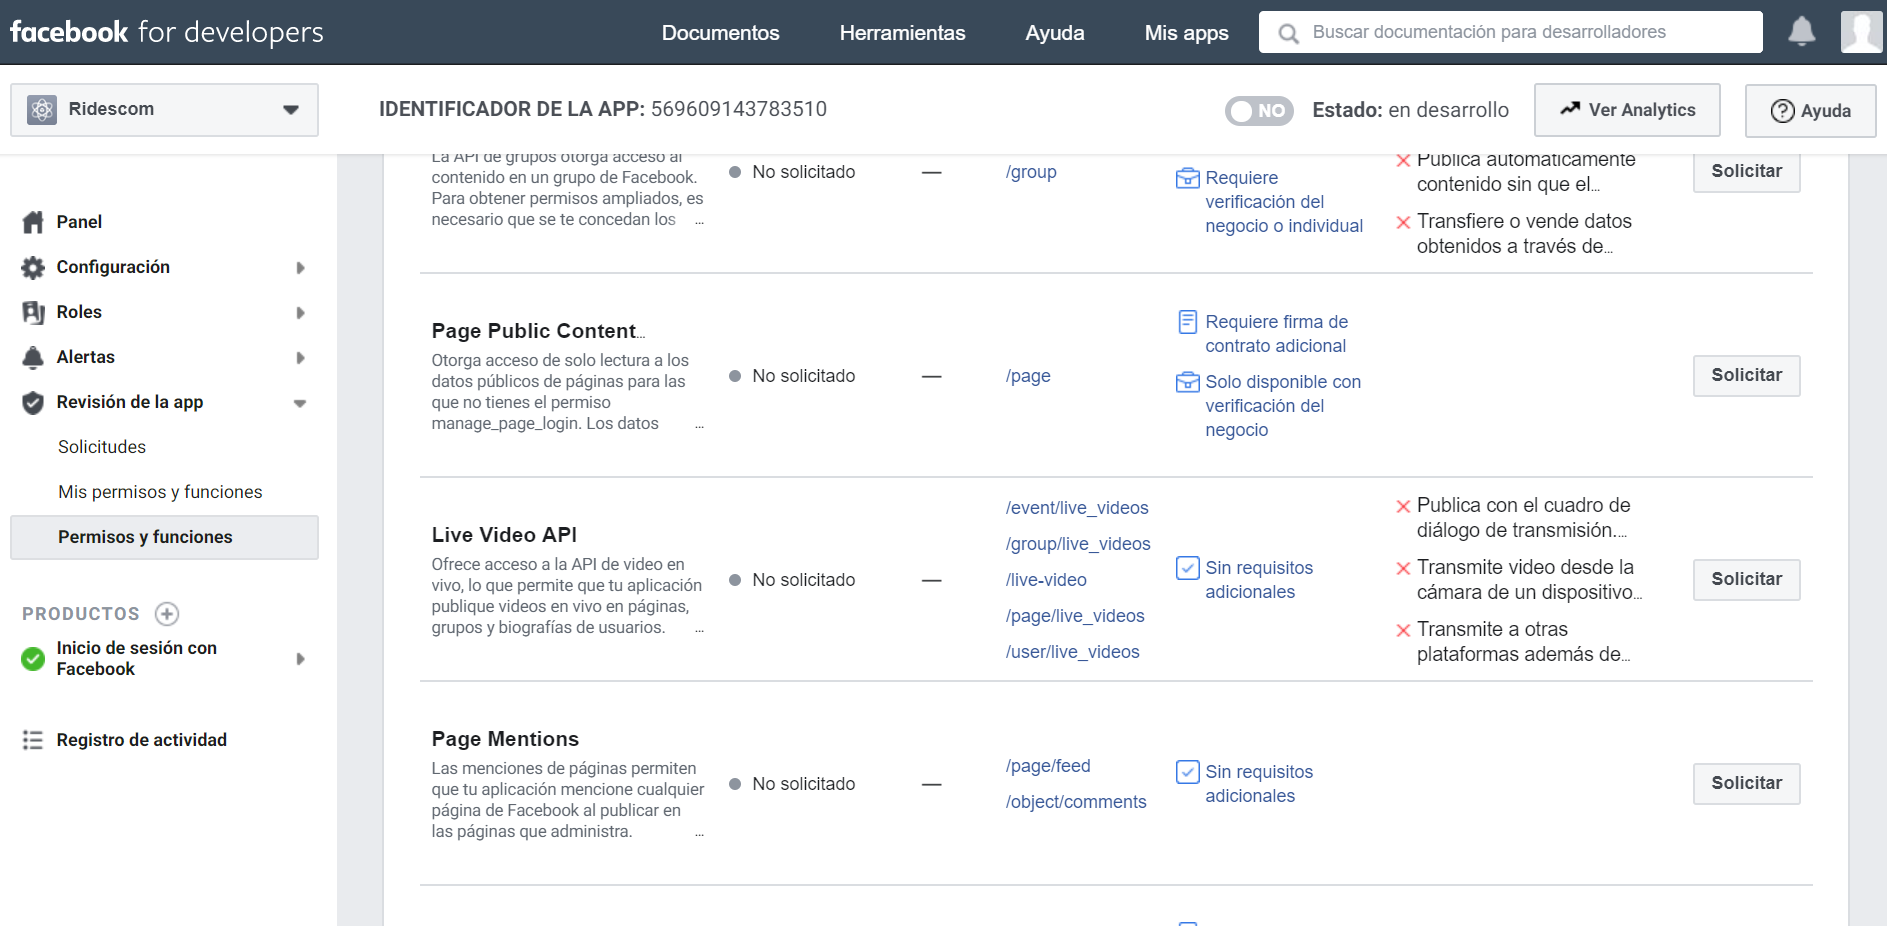
\includegraphics[width=10cm, height=6cm]{Imagenes/FacebookAPI/RequisitoPagina}
		\caption{Requisitos a cumplir para hacer uso de la API de Facebook.}
		\label{requisitosfb}
	\end{figure}
	
	\noindent Dentro de la investigación se encontró que se tenía que seguir paso a paso la
	verificación del negocio y la revisión de la aplicación, con la finalidad de si está todo en orden se
	pueda utilizar las herramientas de Facebook, como se muestra en la siguiente Figura \ref{requisitosfb}. \\
	
	\noindent Realizando la investigación de las actualizaciones para el uso de los plugin de Facebook,
	los datos necesarios para obtener dicha validación, se encontró lo siguiente: \\
	\pagebreak
	
	\textbf{Desarrollo de aplicaciones} \\
	
	En estos documentos, se explica cómo registrar, configurar y desarrollar tu aplicación de modo
	que puedas usar correctamente nuestros productos, API y SDK.
	El ciclo general de desarrollo implica lo siguiente:
	\begin{itemize}
		\item Registrar la aplicación
		\item Seleccionar una situación y agregar productos
		\item Agregar roles
		\item Hacer pruebas en el modo de desarrollo
		\item Solicitar la revisión de aplicaciones
		\item Cambiar al modo activo
	\end{itemize}
	\noindent Repite los pasos Hacer pruebas en el modo de desarrollo y Revisión de
	aplicaciones cada vez que agregues permisos, funciones o productos nuevos o cada vez que
	actualices a una nueva versión de un SDK o de una API.\\
	%https://developers.facebook.com/docs/apps#register
	
	\textbf{Primeros pasos}\\
	Con la API de Pages, las personas pueden actualizar y administrar páginas de Facebook desde su
	aplicación relacionada con la página. Las personas pueden publicar contenido en Facebook o
	Messenger con la identidad de una página. Los casos de uso para API de páginas incluyen:
	\begin{itemize}
		\item Creación de una herramienta de gestión de páginas para clientes o para su
		empresa
		\item Creación de aplicaciones para que los creadores y editores de contenido
		puedan publicar fácilmente como una página
		\item Marketing y publicidad para un negocio utilizando la API de marketing. Para
		obtener más información, consulte API de administración de anuncios y publicaciones de
		páginas no publicadas
		
	\end{itemize}
	%https://developers.facebook.com/docs/pages/getting-started
	
	\textbf{Revisión de apps}\\ 
	
	\noindent Antes de que una app pase a modo activo, es posible que debamos asegurarnos de que
	utilizarás nuestros productos y datos de una manera autorizada. Para lograrlo, requerimos que
	muchas apps se sometan a la revisión de apps.\\
	\noindent En general, el proceso implica especificar el tipo de datos que solicitará la aplicación de
	los usuarios y describir de qué manera utilizará los datos. Según la información que envíes, es
	posible que realicemos un seguimiento y te solicitemos completar otros pasos.\\
	\newline
	¿Cuánto tarda el proceso?\\
	\noindent Por lo general, nos lleva menos de una semana procesar un envío y, con frecuencia, solo
	2 o 3 días. Sin embargo, es posible que tardemos más en períodos pico. Debes tener en cuenta
	que, debido a cambios recientes en el proceso de revisión y al alto volumen de envíos, es posible
	que tardemos varias semanas para completar el proceso de revisión de las apps enviadas.\\
	\newline
	Verificación adicional \\
	\noindent Después de enviar la aplicación para su revisión, es posible que verifiquemos tu	identidad como empresa o como persona. Para hacerlo, te enviaremos una alerta a la bandeja de
	entrada del panel de aplicaciones. La alerta incluirá un enlace para comenzar el proceso de	verificación.\\ %https://developers.facebook.com/docs/apps/review/#supplemental-terms
	
	\noindent Con lo antes investigado se siguió el proceso para verificar la verificación del negocio y
	la comprobación de la aplicación, como se muestra en la siguiente Figura \ref{creacionFB}.
	\pagebreak
	
	\begin{figure}[hbt!]
		\centering
		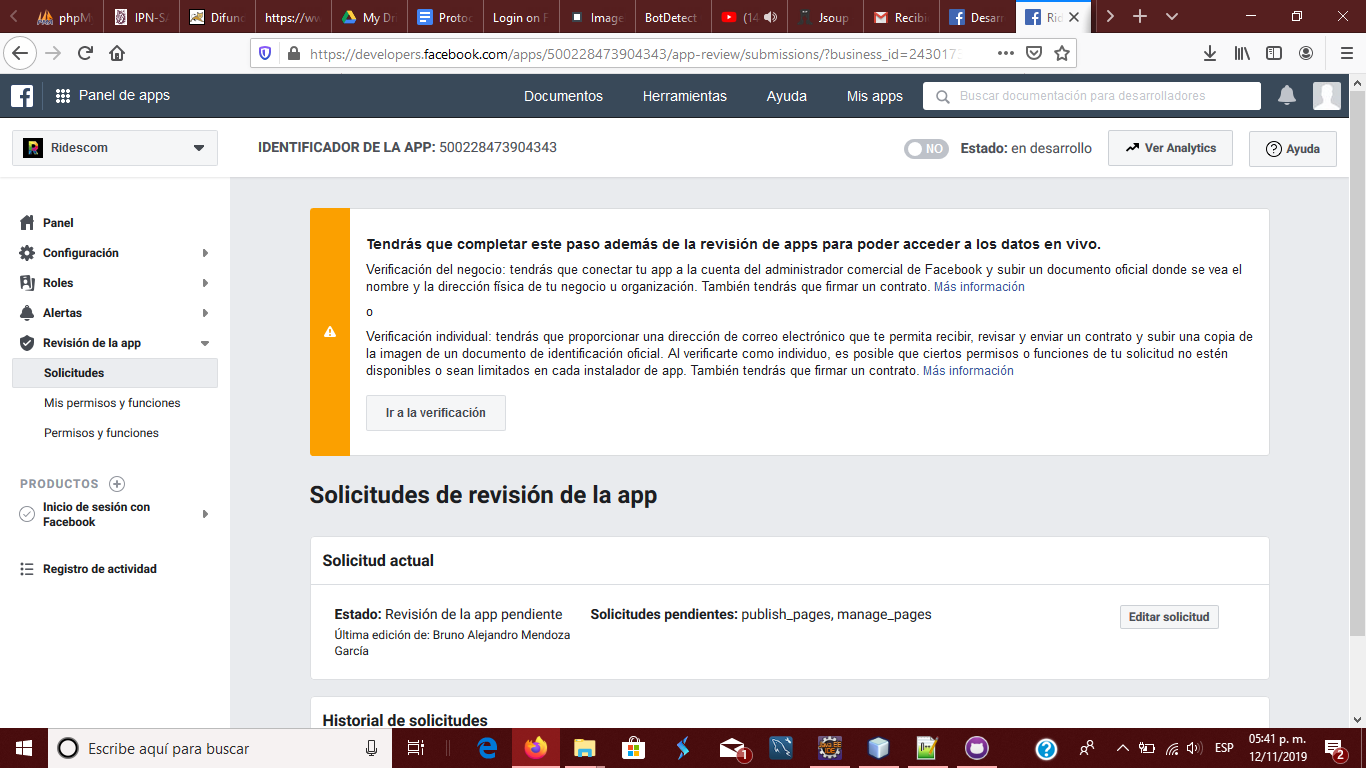
\includegraphics[width=15cm, height=6cm]{Imagenes/FacebookAPI/Facebook1}
		\caption{Solicitud de revisión de app.}
		\label{creacionFB}
	\end{figure}

	\noindent En la Figura \ref{creacionFB2} se muestran los datos necesarios a validar para poder hacer uso del API de Facebook. Especifícamente, la de interés para el proyecto es el API de publish pages.
	\begin{figure}[hbt!]
		\centering
		\includegraphics[width=15cm, height=6cm]{Imagenes/FacebookAPI/Facebook2}
		\caption{Datos a verificar.}
		\label{creacionFB2}
	\end{figure}

	\noindent En la Figura \ref{creacionFB3} se muestra los campos requeridos para poder hacer la solicitud de revisión de la aplicación. Como se puede observar se solicita un icono que identifique a la aplicación, a su vez se solicita una URL en la que se específique las políticas de privacidad, ya que se hace uso de manejo de información personal.
\pagebreak
	\begin{figure}[hbt!]
		\centering
		\includegraphics[width=15cm, height=6cm]{Imagenes/FacebookAPI/Facebook3}
		\caption{Solicitud de datos para revisión de la aplicación.}
		\label{creacionFB3}
	\end{figure}

	\noindent Al ingresar a ver la configuración de la aplicación, en el apartado de solicitudes podemos ver el estatus actual de la solicitud realizada, como se puede apreciar en la Figura \ref{creacionFB7}.

	\begin{figure}[hbt!]
		\centering
		\includegraphics[width=15cm, height=6cm]{Imagenes/FacebookAPI/Facebook7}
		\caption{Estatus de solicitudes.}
		\label{creacionFB7}
	\end{figure}
	
	\noindent En la Figura \ref{creacionFB4} se da una breve descripción de la finalidad de la integración de la API de Facebook en el proyecto desarrollando.
\pagebreak
	\begin{figure}[hbt!]
		\centering
		\includegraphics[width=15cm, height=6cm]{Imagenes/FacebookAPI/Facebook4}
		\caption{Descripción de la finalidad de la aplicación.}
		\label{creacionFB4}
	\end{figure}

	\noindent Como complemento a la solicitud, en la Figura \ref{creacionFB5} se da una breve descripción de la finalidad de la solicitud manage pages.

	\begin{figure}[hbt!]
		\centering
		\includegraphics[width=15cm, height=6cm]{Imagenes/FacebookAPI/Facebook5}
		\caption{Descripción del uso de manage page en la aplicación desarrollando.}
		\label{creacionFB5}
	\end{figure}

	\noindent Al completar los campos requeridos nos muestra un mensaje de confirmación de la solicitud de revisión, como se muestra en la Figura \ref{creacionFB15}
\pagebreak
	\begin{figure}[hbt!]
		\centering
		\includegraphics[width=15cm, height=6cm]{Imagenes/FacebookAPI/Facebook15}
		\caption{paso 15}
		\label{creacionFB15}
	\end{figure}

	\noindent Una vez completado los pasos anteriores, nos es re dirigido a la página donde se visualizan las aplicaciones que se tienen, como se puede ver en la Figura \ref{creacionFB6}.
	\begin{figure}[hbt!]
		\centering
		\includegraphics[width=15cm, height=6cm]{Imagenes/FacebookAPI/Facebook6}
		\caption{Solicitud completada}
		\label{creacionFB6}
	\end{figure}
	
	\noindent En la Figura \ref{creacionFB8}, se puede visualizar la configuración actual de la aplicación. De tal manera que se visualiza que no existe algún dato faltante.

	\begin{figure}[hbt!]
		\centering
		\includegraphics[width=15cm, height=6cm]{Imagenes/FacebookAPI/Facebook8}
		\caption{Configuración de la aplicación.}
		\label{creacionFB8}
	\end{figure}
\pagebreak
	
	En la Figura \ref{creacionFB9}, se puede observar el estatus de la solicitud de la información individual. En esta se solicitó información acerca de la persona que estaba desarrollando la aplicación.
	\begin{figure}[hbt!]
		\centering
		\includegraphics[width=15cm, height=6cm]{Imagenes/FacebookAPI/Facebook9}
		\caption{Estatus solicitud individual.}
		\label{creacionFB9}
	\end{figure}

	En la Figura \ref{creacionFB11}, se puede observar el estatus de la verificación del negocio. En este se solicitaron datos acerca de la empresa para la cual se estaba creando el proyecto, que en nuestro caso se envió la información acerca del Trabajo Terminal.
	\begin{figure}[hbt!]
		\centering
		\includegraphics[width=15cm, height=6cm]{Imagenes/FacebookAPI/Facebook11}
		\caption{Estatus Solicitud Negocio.}
		\label{creacionFB11}
	\end{figure}
\pagebreak
	Al terminar de revisar el estatus individual de cada requisito, se muestra de manera gráfica el proceso actual de la o las solicitudes realizadas. En está se puede apreciar que el tiempo estimado en la que se proporcionaría una respuesta es en 5 días, como se muestra en la Figura \ref{creacionFB12}.

	\begin{figure}[hbt!]
		\centering
		\includegraphics[width=15cm, height=6cm]{Imagenes/FacebookAPI/Facebook12}
		\caption{Gráfica de estatus de solicitud.}
		\label{creacionFB12}
	\end{figure}
\pagebreak
	\noindent Al pasar los 5 días en los que se revisaba la solicitud, se notifica que es requisito el enviar datos mucho más especifícos del negocio u organización, como se muestra en la Figura \ref{creacionFB16}. Siendo en este primer punto un factor de incertidumbre ya que al tratarse de un proyecto escolar, el envío de estos datos pueda repercutir en temas mucho más sencibles.

	\begin{figure}[hbt!]
		\centering
		\includegraphics[width=15cm, height=6cm]{Imagenes/FacebookAPI/Facebook16}
		\caption{Respuesta a solititud.}
		\label{creacionFB16}
	\end{figure}
	
	
	\chapter{Apartado H: Base de Datos}
	\noindent En este apartado, se muestra la estructura de la base de datos que tiene la aplicación web. Se tomó en consideración los requisitos y problemática que se tenían para proporcionar una respuesta óptima de los datos. Cabe mencionar que la base de datos se modeló para que esta pueda funcionar cuando al proyecto se agreguen más unidades académicas.
	
		\label{BasedeDatos}
		\begin{figure}[hbt!]
			\centering
			\includegraphics[angle=90, width=14cm, height=19cm]{Imagenes/RIDESCOM.png}
			\caption{Estructura de la Base de Datos de RIDESCOM}
			\label{BaseDatos}
		\end{figure}
		
		
	
	\pagebreak
		
	\chapter{Apartado I: Vistas}
	\noindent En este apartado, se muestran las vistas finales de la aplicación web, mostrando cada uno de los módulos junto con su descripción y al actor que corresponde cada una de ellas.
		
		\begin{figure} [hbt!]
			\centering
			\includegraphics[width=10cm, height=6cm]{Imagenes/Vistas/VIsta1_TipoSesion}
			\caption{Vista que ayuda a definir el tipo de usuario que ingresará.}
			\label{VistaTipoSesion}
		\end{figure}
	
		\begin{figure} [hbt!]
			\centering
			\includegraphics[width=10cm, height=6cm]{Imagenes/Vistas/Vista2_InicioSesionJFD}
			\caption{Vista del Inicio de Sesión para el Jefe de Fomento Deportivo y el Coordinador de una Unidad Académica.}
			\label{VistaInicioSesionJFD}
		\end{figure}
	
		\begin{figure} [hbt!]
			\centering
			\includegraphics[width=10cm, height=6cm]{Imagenes/Vistas/Vista3_PrincipalJFD}
			\caption{Vista principal del Jefe de Fomento Deportivo (JFD).}
			\label{VistaPrincipalJFD}
		\end{figure}
			
		\begin{figure} [hbt!]
			\centering
			\includegraphics[width=10cm, height=6cm]{Imagenes/Vistas/Vista4_PrincipalJFD}
			\caption{Vista principal del Jefe de Fomento Deportivo continuación(JFD).}
			\label{VIstaPrincipalJFD1}
		\end{figure}
	
		\begin{figure} [hbt!]
			\centering
			\includegraphics[width=10cm, height=6cm]{Imagenes/Vistas/Vista5_MenuUsuarioJFD}
			\caption{Vista que muestra datos del usuario en sesión.(Jefe de Fomento Deportivo)}
			\label{VistaMenuUsuario}
		\end{figure}
		
		\begin{figure} [hbt!]
			\centering
			\includegraphics[width=10cm, height=6cm]{Imagenes/Vistas/Vista6_ConsultaCoordJFD}
			\caption{Vista donde se visualizan los Coordinadores de Unidades Académicas registrados.}
			\label{VistaConsultaCoord}
		\end{figure}
		
		\begin{figure} [hbt!]
			\centering
			\includegraphics[width=10cm, height=6cm]{Imagenes/Vistas/Vista7_DeportesJFD}
			\caption{Vista en la que el Jefe de Fomento Deportivo visualiza los deportes que se practican actualmente en el Instituto Politécnico Nacional.}
			\label{VistaDeportes}
		\end{figure}
		
		\begin{figure} [hbt!]
			\centering
			\includegraphics[width=10cm, height=6cm]{Imagenes/Vistas/Vista8_PruebaJFD}
			\caption{Vista donde el Jefe de Fomento Deportivo podrá ver las pruebas que han sido registradas.}
			\label{VistaPruebas}
		\end{figure}
	
		\begin{figure}
			\centering
			\includegraphics[width=10cm, height=6cm]{Imagenes/Vistas/Vista20_AgregaPrueba}
			\caption{Vista para agregar una prueba.}
			\label{VistaAgregaPrueba}
		\end{figure}
		
	
		\begin{figure} [hbt!]
			\centering
			\includegraphics[width=10cm, height=6cm]{Imagenes/Vistas/Vista9_SedesJFD}
			\caption{Vista para visualizar las sedes donde se llevarán a cabo los eventos interpolitécnicos deportivos.}
			\label{VistaSedes}
		\end{figure}
		
		\begin{figure} [hbt!]
			\centering
			\includegraphics[width=10cm, height=6cm]{Imagenes/Vistas/Vista10_AgregaEvento}
			\caption{Vista en la que se puede agregar un Evento Interpolitécnico Deportivo.}
			\label{VistaAgregarEvento}
		\end{figure}
	
		\begin{figure} [hbt!]
			\centering
			\includegraphics[width=10cm, height=6cm]{Imagenes/Vistas/Vista11_EditarEvento}
			\caption{Vista en la que se pueden editar los datos de un Evento Interpolitécnico Deportivo.}
			\label{VistaEditarEvento}
		\end{figure}
		
		\begin{figure} [hbt!]
			\centering
			\includegraphics[width=10cm, height=6cm]{Imagenes/Vistas/Vista12_PrincipalCoord}
			\caption{Vista principal del Coordinador de la Unidad Académica.}
			\label{VistaPrincipalCoord}
		\end{figure}
		
		\begin{figure} [hbt!]
			\centering
			\includegraphics[width=10cm, height=6cm]{Imagenes/Vistas/Vista13_PrincipalCoord}
			\caption{Vistas principal del Coordinador de la Unidad Académica. (Continuación)}
			\label{VistaPrincipalCoord1}
		\end{figure}
		
		\begin{figure} [hbt!]
			\centering
			\includegraphics[width=10cm, height=6cm]{Imagenes/Vistas/Vista14_MenuUsuarioCoord}
			\caption{Vista que muestra datos del usuario en sesión.(Coordinador)}
			\label{VistaMenuCoord}
		\end{figure}
		
		\begin{figure} [hbt!]
			\centering
			\includegraphics[width=10cm, height=6cm]{Imagenes/Vistas/Vista15_ConsultaEntrenador}
			\caption{Vista para la consulta de entrenadores.}
			\label{VistaConsultaEntrenador}
		\end{figure}
		
		\begin{figure} [hbt!]
			\centering
			\includegraphics[width=10cm, height=6cm]{Imagenes/Vistas/Vista16_AgregaEntrenador}
			\caption{Vista para agregar a un entrenador.}
			\label{VistaAgregarEntrenador}
		\end{figure}
	
		\begin{figure} [hbt!]
			\centering
			\includegraphics[width=10cm, height=6cm]{Imagenes/Vistas/Vista17_EditarEntrenador}
			\caption{Vista para editar los datos del entrenador.}
			\label{VistaEditarEntrenador}
		\end{figure}
		
		\begin{figure} [hbt!]
			\centering
			\includegraphics[width=10cm, height=6cm]{Imagenes/Vistas/Vista18_ConsultaInscritos}
			\caption{Vista para consultar los alumnos inscritos en algún Evento Interpolitécnico Deportivo.}
			\label{VistaConsultaInscritos}
		\end{figure}
		
		\begin{figure} [hbt!]
			\centering
			\includegraphics[width=10cm, height=6cm]{Imagenes/Vistas/Vista19_ConsultaResultados}
			\caption{Vista para consultar los resultados obtenidos por los participantes.}
			\label{VistaConsultaResultados}
		\end{figure}
		
		
